%%----------------------------------------------------------------------------------
% DO NOT Change this is the required setting A4 page, 11pt, onside print, book style
%%----------------------------------------------------------------------------------
\documentclass[a4paper,11pt,oneside]{book} 
\usepackage{CS_report} % DO NOT REMOVE THIS LINE. 
%%%%%%%%%%%%%%%%%%%%%%%%%%%%%%%%%%%%%%%%%%%%%%%%%%%%%%%%%%%%%%%%%%%%%%%%%%%%%%%%%%%%


%%%%%%%%%%%%%%%%%%%%%%%%%%%%%%%%%%%%%%%%%%%%%%%%%%%%%%%%%%%%%%%%%%%%%%%%%%%%%%%%%%%%
\begin{document}
    \captionsetup[figure]{margin=1.5cm,font=small,name={Figure},labelsep=colon}
    \captionsetup[table]{margin=1.5cm,font=small,name={Table},labelsep=colon}
    
    \frontmatter
    
    %%%%%%%%%%%%%%%%%%%%%%%%%%%%%%%%%%%%%%%%%%%%%%%%%%%%%%%%%%%%%%%%%%%%%%%%%%%%%%%%
    \begin{titlepage}      
        \begin{center}
            % Comment out UoR logo if not applicable
            
\includegraphics[width=7cm]{figures/UDLogo.png}\\[0.3cm]
            {\LARGE Universidad Distrital Francisco José de Caldas\\[0.3cm]
            Computer Engineering Program\\[0.3cm]
            School of Engineering}\\[2cm]
			
            \linespread{1.0}\huge {
                Workshop No. 2 -- Kaggle Project Analysis: CIBMTR Equity in Post-HCT Survival Predictions
            }
            \linespread{1}~\\[2cm]
            {\Large 
                Sergio Nicolás Mendivelso Martínez -- 20231020227\\
                Sergio Leonardo Moreno Granado -- 20242020091\\
                Juan Manuel Otálora Hernández -- 20242020018\\
                Juan Diego Moreno Ramos -- 20242020009\\
            }
            

            {\Large 
                \emph{Professor:} Eng. Carlos Andrés Sierra, M.Sc.}\\[1cm]
            
    		\large A report submitted for Workshop No. 2 in Systems Analysis \& Design\\
            Semester 2025-III 
            \\[0.3cm] 
            \vfill
            
            
            October 2025, Bogotá D.C.
        \end{center}
    \end{titlepage}

     
    % -------------------------------------------------------------------
    % Abstract and Acknowledgement
    % -------------------------------------------------------------------
    
    % -------------------------------------------------------------------
	% Acknowledgement
	% -------------------------------------------------------------------
    
    % -------------------------------------------------------------------
    % Contents, list of figures, list of tables
    % -------------------------------------------------------------------
    
    \tableofcontents
    \listoffigures
    %\listoftables
    %\input{glossaries} % List abbreviations: e.g., HCT: Hematopoietic Cell Transplantation, EFS: Event-Free Survival, C-index: Concordance Index.

    %%%%%%%%%%%%%%%%%%%%%%%%%%%%%%%%%%%%%%%%%%%%%%%%%%%%%%%%%%%%%%%%%%%%%%%
    %%                                                                    %%  
    %%  Main chapters and sections of your project                        %%  
    %%  Everything from here on needs updates in your own words and works %%
    %%                                                                    %%
    %%%%%%%%%%%%%%%%%%%%%%%%%%%%%%%%%%%%%%%%%%%%%%%%%%%%%%%%%%%%%%%%%%%%%%%%
    \mainmatter
    
    %\chapter{Introduction and System Analysis}

\section{Overview}

The ``CIBMTR – Equity in Post-HCT Survival Predictions'' competition has as its primary objective the development of models that accurately predict survival outcomes after allogeneic hematopoietic cell transplantation (HCT) \cite{kaggle_competition}. What distinguishes this competition is its dual approach: predictions must not only be accurate but also equitable, addressing existing disparities by ensuring that models do not disadvantage patients based on their demographic or socioeconomic background.

\vspace{0.3cm}

The provided dataset contains clinical, genetic, and demographic information for each patient. Relevant variables include age, ethnicity, disease risk indices, genetic compatibility metrics, and detailed medical histories \cite{cibmtr_datasets}. By leveraging this multifaceted data, the goal is to promote innovations in predictive modeling that can directly inform and improve personalized medicine and transplant care.

\vspace{0.3cm}

The main competition rules are as follows: Data use is strictly limited to the datasets provided within the competition framework; external data is not permitted unless explicitly authorized. Additionally, participants must meet equity criteria, as solutions will be evaluated not only for their overall accuracy but also for their equitable performance across different patient groups \cite{kaggle_competition}.

\vspace{0.3cm}

\section{Objectives}

This workshop aims to achieve the following interconnected objectives:
\begin{itemize}
    \item Understand the structure of the competition's system
    \item Learn more about the medical context to apply new ideas as accurately as possible
    \item Identify the system's elements, relationships, and boundaries
    \item Check the sensitivity and complexity of the problem
    \item Analyze the evaluation metric
    \item Propose recommendations to improve the accuracy and fairness of the models
\end{itemize}

\section{Medical Background}

\subsection{Allogeneic Hematopoietic Cell Transplantation}

Allogeneic Hematopoietic Cell Transplantation (HCT) is a medical procedure where a patient receives healthy blood stem cells from a compatible donor \cite{uptodate_hct}. These new cells replace the patient's damaged or sick bone marrow and help rebuild a working blood and immune system. Recent advances in transplantation have significantly improved patient survival over time, though high morbidity and mortality risks remain critical challenges \cite{astct_simplification}.

The term allogeneic means the cells come from another person (a relative or someone unrelated). Although stem cells can be collected in different ways, bone marrow remains a primary source for transplantation \cite{aacr_historical}.

This procedure is mainly used to treat serious blood and immune system diseases, such as:
\begin{itemize}
    \item Acute and chronic leukemias \cite{ash_transplant_all}
    \item Lymphomas
    \item Multiple myeloma
    \item Severe aplastic anemia
    \item Immune disorders \cite{biorxiv_autoimmune}
\end{itemize}

The goal is to replace faulty or harmful cells with stem cells that can create healthy new blood cells like red blood cells, white blood cells (T and B lymphocytes), and platelets \cite{uptodate_hct}.

\subsection{The Transplantation Process}

The HCT process involves several critical stages \cite{uptodate_hct}:

\begin{enumerate}
    \item \textbf{Donor selection:} A genetic compatibility test (HLA typing) is performed. The better the match, the lower the risk of rejection. This is where prediction models from the competition become relevant.
    
    \item \textbf{Patient preparation:} Before the transplant, the patient receives chemotherapy and/or radiation to:
    \begin{itemize}
        \item Destroy diseased cells
        \item Suppress the immune system to prevent rejection
    \end{itemize}
    
    \item \textbf{Stem cell infusion:} The transplant is not a surgical procedure. Stem cells are administered through an IV, similar to a blood transfusion.
    
    \item \textbf{Engraftment:} The donor's stem cells travel to the patient's bone marrow and begin producing new blood cells. Recent studies have shown that robust and polyclonal engraftment occurs across different age groups, though with distinct differences in cellular diversity \cite{stmcls_clonality}.
    
    \item \textbf{Follow-up:} Patients require close monitoring to detect and manage complications.
\end{enumerate}

\subsection{Risks and Complexity}

Because the transplant uses cells from another person, there is a risk that the patient's body may recognize them as foreign. Laboratory tests are conducted to reduce the likelihood of rejection or immune reactions \cite{uptodate_gvhd}.

Possible complications include:
\begin{itemize}
    \item \textbf{Graft-versus-host disease (GVHD):} The donor's immune cells may attack the patient's tissues \cite{uptodate_gvhd, ash_chronic_gvhd}
    \item \textbf{Infections}
    \item \textbf{Graft failure:} The new cells fail to engraft or function properly
    \item \textbf{Social and geographic factors:} These can affect access to care, treatment follow-up, and overall outcomes \cite{mdpi_cancers}
\end{itemize}

\subsection{Importance of Survival Prediction}

Allogeneic transplants are high-risk and expensive procedures \cite{astct_simplification}. Accurate survival prediction:
\begin{itemize}
    \item Helps physicians make better decisions about transplant candidacy
    \item Enables more personalized treatment and care protocols
    \item Improves utilization of healthcare resources
    \item Reduces health inequalities, as current models often favor certain population groups \cite{jama_ai_medicine}
\end{itemize}

\section{System Analysis}

\subsection{Input Data Sources and Characteristics}

The predictive system incorporates comprehensive data sources spanning clinical, transplant-specific, demographic, and temporal dimensions:

\subsubsection{Disease and Clinical Characteristics}
\begin{itemize}
    \item Disease characteristics: Type of hematological malignancy, disease stage at transplant, remission status
    \item Pre-transplant comorbidity indices: Existing health conditions that affect transplant outcomes
    \item Previous treatment history: Chemotherapy cycles, radiation exposure, prior transplants
    \item Laboratory values: Blood counts, organ function markers, inflammatory markers
    \item Karnofsky/Lansky performance scores: Functional status indicators
\end{itemize}

\subsubsection{Transplant-Specific Inputs}
\begin{itemize}
    \item Donor type: Matched related, matched unrelated, haploidentical, cord blood
    \item HLA matching degree: Level of compatibility between donor and recipient
    \item Stem cell source: Bone marrow, peripheral blood, umbilical cord
    \item Conditioning regimen intensity: Myeloablative, reduced intensity, non-myeloablative
    \item Graft-versus-host disease prophylaxis protocol
\end{itemize}

\subsubsection{Demographic and Socioeconomic Inputs}
\begin{itemize}
    \item Age at transplant (continuous variable)
    \item Sex/gender (categorical)
    \item Race/ethnicity (categorical, critical for equity analysis)
    \item Geographic location (affects access to care)
    \item Insurance status (impacts follow-up care quality)
\end{itemize}

\subsubsection{Temporal Inputs}
\begin{itemize}
    \item Year of transplant (captures medical advances over time)
    \item Time from diagnosis to transplant (affects disease progression)
    \item Follow-up duration markers
\end{itemize}

\subsection{System Architecture and Modules}

The predictive system employs a sophisticated modular architecture designed to ensure both accuracy and equity in survival predictions:

\subsubsection{Data Preprocessing Module}
This module handles initial data preparation through multiple stages:
\begin{itemize}
    \item Feature engineering: Creating interaction terms between clinical and demographic variables, calculating risk scores from raw measurements, generating time-dependent features
    \item Data standardization and normalization while preserving demographic-related variations that might mask inequities
    \item Handling missing data and outliers with equity-aware imputation methods
\end{itemize}

\subsubsection{Equity Analysis Module}
This component specifically addresses fairness in the model:
\begin{itemize}
    \item Stratified analysis across demographic groups to identify potential biases
    \item Bias detection algorithms measuring disparities in data quality, feature availability, and baseline outcome rates
    \item Fairness-aware preprocessing techniques, such as reweighting samples to balance representation across demographic groups while preserving clinical validity
\end{itemize}

\subsubsection{Feature Selection and Importance Module}
This system component determines which variables contribute most to survival predictions:
\begin{itemize}
    \item Multiple selection strategies: Clinical domain knowledge integration, statistical significance testing, machine learning-based feature importance rankings
    \item Ensuring predictive features are available equitably across all patient populations
    \item Avoiding features that might be systematically missing for certain demographic groups
\end{itemize}

\subsubsection{Predictive Modeling Core}
The central prediction engine employs an ensemble approach:
\begin{itemize}
    \item Survival analysis models: Cox proportional hazards and accelerated failure time models for time-to-event predictions
    \item Machine learning algorithms: Gradient boosting machines and random forests for complex pattern recognition
    \item Deep learning architectures for capturing non-linear relationships
    \item Cross-validation specifically designed for survival data with demographic stratification
\end{itemize}

\subsubsection{Fairness Calibration Module}
This post-processing component adjusts model predictions for equitable performance:
\begin{itemize}
    \item Calibration techniques maintaining similar prediction accuracy across different patient populations
    \item Threshold optimization considering fairness metrics alongside traditional performance measures
    \item Disparity impact assessment to quantify and minimize prediction inequities
\end{itemize}

\subsubsection{Uncertainty Quantification Module}
This component provides confidence intervals and prediction uncertainties:
\begin{itemize}
    \item Prediction intervals using techniques appropriate for survival analysis
    \item Risk stratification with associated uncertainty bounds
    \item Identification of cases where predictions might be less reliable due to data limitations
\end{itemize}

\subsection{System Outputs}

The system generates comprehensive outputs for clinical decision support and equity monitoring:

\subsubsection{Primary Output}
\begin{itemize}
    \item Survival Probability Predictions: Time-dependent survival probabilities at key clinical milestones (100 days, 1 year, 2 years, 5 years post-transplant)
    \item Risk Stratification Categories: Patient classification into risk groups (low, intermediate, high) with associated survival curves
\end{itemize}

\subsubsection{Secondary Outputs}
\begin{itemize}
    \item Equity Metrics Dashboard: Comprehensive fairness assessments including demographic parity measures showing prediction consistency across groups
    \item Clinical Decision Support Outputs: Individualized risk factors highlighting important predictors, comparative analysis showing patient risk profiles, treatment modification suggestions based on modifiable risk factors
    \item Model Interpretability Outputs: Feature importance rankings, partial dependence plots, SHAP values providing detailed explanations for individual predictions
    \item Quality Assurance Outputs: Model performance metrics, calibration plots, data quality reports identifying input data issues
    \item Research and Monitoring Outputs: Aggregate statistics for clinical research, temporal trend analyses, center-specific performance metrics for transplant program evaluation
\end{itemize}

\section{Complexity and Sensitivity Analysis}

\subsection{Complexity in Post-HCT Survival Modeling}

The challenge of predicting survival outcomes after hematopoietic cell transplantation (HCT) lies fundamentally in the system's complexity \cite{astct_simplification}. Multiple interconnected clinical, genetic, and demographic factors influence patient survival, from age, disease stage, and comorbidities to donor compatibility and care protocols. The interaction of these variables forms a nonlinear, high-dimensional system where unexpected effects can arise from subtle parameter changes \cite{frontiers_ai_hct}.

\vspace{0.3cm}

Furthermore, feedback effects, such as immune responses, transplant complications, or secondary interventions, can introduce new layers of complexity, making simple models insufficient to capture the true patient trajectory \cite{stmcls_clonality}.

\subsection{Sensitivity Analysis}

Small variations in input variables can cause significant differences in survival predictions. For example, changing a patient's age or disease risk index value can substantially modify the survival estimate, relocating the patient to another risk group or altering their prognosis \cite{mdpi_cancers}. Similarly, the presence or absence of certain comorbidities (such as renal failure or previous infections) can generate major changes in the final model outcome.

\vspace{0.3cm}

A technique used to measure this complexity is subgroup analysis, whereby dividing the sample into subgroups (by age, gender) and examining how predictions change can analyze the system's sensitivity to these changes.

\textbf{Sensitive parameters include:}
\begin{itemize}
    \item \textbf{Age:} An increase of only one year can move a patient from a low to high-risk category \cite{stmcls_clonality}
    \item \textbf{Disease risk index:} Small changes in the score can alter prognosis or eligibility for specific treatments
    \item \textbf{Genetic compatibility:} Minimal differences can affect transplant rejection rates and survival
    \item \textbf{Severe comorbidities:} Their presence or absence can double or drastically reduce projected survival
\end{itemize}

\subsection{Chaos and Randomness in Post-HCT Survival Prediction}

Medical outcomes following allogeneic hematopoietic cell transplantation (HCT) are intrinsically unpredictable and complex, with many processes exhibiting characteristics of chaos and randomness \cite{frontiers_ai_hct}. Chaos theory, which describes how small variations in initial conditions can lead to vastly different outcomes, is highly relevant for survival modeling in this context. Even small inaccuracies or variations in clinical measurements, such as patient age, genetic compatibility, or comorbidities, can dramatically change survival predictions.

\vspace{0.3cm}

This sensitivity is sometimes known as the ``butterfly effect'' in nonlinear systems. Randomness also plays a key role. Patient data contain elements of stochasticity arising from biological diversity, incomplete records, and unknown confounding factors \cite{biorxiv_autoimmune}. For example, two patients with apparently identical risk factors may experience completely different outcomes after transplantation due to hidden genetic or environmental variables.

\vspace{0.3cm}

Therefore, the proposed model must be robust against noise, outliers, and missing data, as these introduce additional layers of unpredictability in survival outcomes. Furthermore, feedback loops and nonlinearities, such as immune responses or treatment complications, can give rise to emergent behaviors that are difficult to predict using traditional linear models \cite{frontiers_immunology}. These dynamic interactions illustrate how system evolution cannot be fully explained or predicted by examining its individual parts in isolation. Even the most advanced predictive models may struggle to capture all aspects of post-HCT survival, highlighting the ever-present influence of chaos and randomness in personalized medicine.

\section{Evaluation and Metrics}

\subsection{The C-Index Metric}

The C-Index is a metric used to evaluate a survival model's ability to correctly order risk among pairs of patients \cite{kaggle_competition}. In the Kaggle competition on post-HCT survival, a ``stratified'' version is used, meaning the C-index is calculated within each racial group of patients and then these results are averaged with dispersion adjustment. This stratified C-Index dictates that our model must be not only accurate overall but consistent and fair across all ethnic subgroups present in the dataset.

\subsection{Importance of Equity in Medical Predictions}

Equity in medical predictions is fundamental because it ensures that all patients, regardless of their race, gender, socioeconomic status, or other factors, receive fair and accurate care \cite{jama_ai_medicine}. When predictive models do not consider equity, they can perpetuate existing inequalities in the health system.

\section{Visual Representation}

\begin{figure}[htbp]
    \centering
    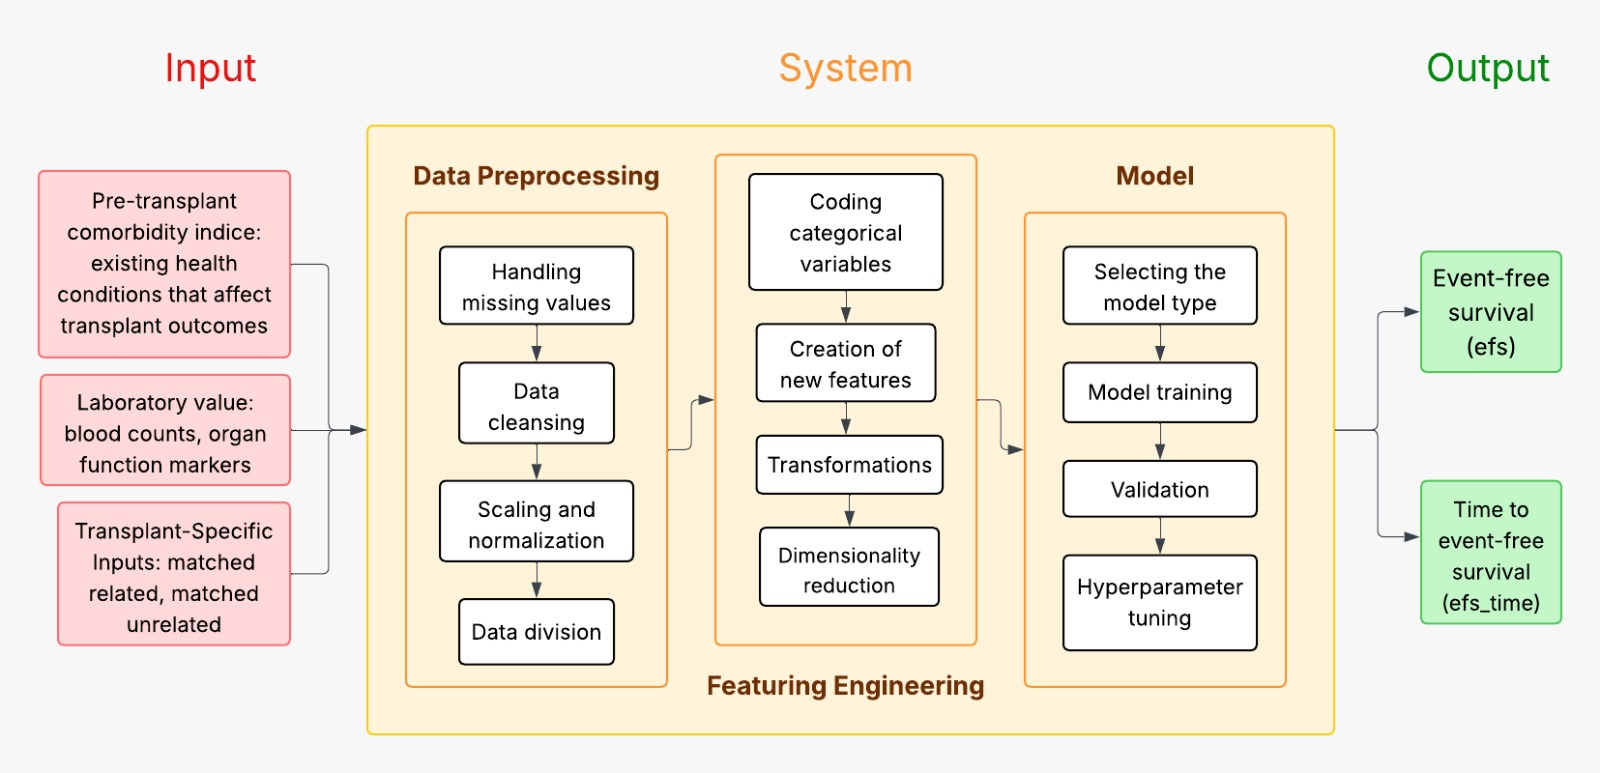
\includegraphics[width=1\textwidth]{figures/SystemDiagram.jpg}
    \caption{Diagram illustrating the modular pipeline of the predictive system. The diagram shows the flow from input data sources through preprocessing, equity analysis, feature selection, predictive modeling, fairness calibration, and uncertainty quantification modules, culminating in the output of survival predictions and equity metrics.}
    \label{fig:system_architecture}
\end{figure}

\section{Conclusions}

\subsection{Key Findings Summary}

This analysis reveals several critical aspects of the CIBMTR competition system:

\begin{itemize}
    \item The complexity of post-HCT survival prediction stems from multiple interacting clinical, demographic, and transplant-specific factors
    \item The modular system architecture enables both accurate predictions and equitable performance across demographic groups
    \item Small parameter variations can significantly impact predictions, requiring robust sensitivity analysis
    \item The stratified C-index metric ensures equitable model performance while maintaining clinical accuracy
    \item System sensitivity requires sophisticated modeling approaches with built-in fairness calibration
\end{itemize}

\subsection{System Strengths and Weaknesses}

\textbf{Strengths:}

\begin{itemize}
    \item Comprehensive multi-modular architecture addressing both accuracy and equity \cite{kaggle_competition}
    \item Integrated fairness calibration throughout the prediction pipeline
    \item Real-world medical application with high impact potential \cite{astct_simplification}
    \item Sophisticated handling of clinical complexity through ensemble modeling approaches \cite{frontiers_ai_hct}
    \item Comprehensive output system supporting clinical decision-making and equity monitoring
\end{itemize}

\textbf{Weaknesses:}

\begin{itemize}
    \item High system complexity requires substantial computational resources
    \item Inherent randomness and chaos in biological systems \cite{biorxiv_autoimmune}
    \item Potential for hidden confounding variables not captured in current data sources
    \item Dependence on data quality and completeness across all demographic groups
    \item Challenges in generalizing across different healthcare systems and populations
\end{itemize}

\subsection{Recommendations}

To improve accuracy and equity in predictions:

\begin{itemize}
    \item Implement advanced ensemble methods to handle system complexity while maintaining interpretability \cite{frontiers_ai_hct}
    \item Develop cross-validation strategies that maintain demographic balance across all folds
    \item Create robust preprocessing techniques specifically designed for clinical missing data patterns
    \item Incorporate domain expertise in feature engineering to ensure clinical relevance
    \item Apply fairness-aware regularization techniques to prevent overfitting to majority groups
    \item Consider temporal dynamics and evolving medical practices in patient outcomes \cite{stmcls_clonality}
    \item Enhance uncertainty quantification to support clinical decision-making under uncertainty
\end{itemize}

\subsection{Clinical and Healthcare System Implications}

This work has significant implications for:

\begin{itemize}
    \item Enhanced clinical decision-making in transplant medicine through personalized risk assessment \cite{astct_simplification}
    \item More equitable allocation of medical resources based on accurate and fair predictions
    \item Advancement of personalized medicine approaches through comprehensive risk profiling \cite{biorxiv_autoimmune}
    \item Reduction of healthcare disparities through systematic bias detection and mitigation \cite{jama_ai_medicine}
    \item Development of fair AI systems in healthcare that can be trusted across diverse populations
    \item Improved patient outcomes through better risk stratification and targeted interventions
    \item Quality improvement in transplant programs through comprehensive monitoring and evaluation outputs
\end{itemize} % Paste Introduction content: Brief context, importance, objectives (Comprender la estructura..., etc.).

     \chapter{System Design}

\section{Review of Workshop No. 1 Findings}
\subsection{Summary of Systems Analysis}

In Workshop 1, we conducted a comprehensive systems analysis of the CIBMTR Kaggle competition focused on equity in post-HCT survival predictions. Our analysis revealed the complex nature of the medical system surrounding hematopoietic cell transplantation procedures, characterized by multiple interconnected clinical, genetic, and demographic factors that influence patient outcomes.

Key findings from our analysis include:

\begin{itemize}
    \item \textbf{System Components:} The system comprises diverse data sources including disease characteristics, transplant-specific inputs, demographic factors, and temporal variables, all contributing to survival predictions.
    
    \item \textbf{High Complexity:} Post-HCT survival prediction involves nonlinear interactions between variables, forming a high-dimensional system where small parameter changes can lead to significant outcome differences.
    
    \item \textbf{Sensitivity Analysis:} We identified critical sensitivity parameters including patient age, disease risk indices, genetic compatibility scores, and comorbidities, where minor variations can dramatically alter survival predictions.
    
    \item \textbf{Chaos Theory:} Medical outcomes following HCT exhibit characteristics of chaos theory and inherent randomness, where small inaccuracies in measurements can lead to unpredictable outcomes.
    
    \item \textbf{Equity Considerations:} The stratified C-index metric ensures model performance is consistent across ethnic subgroups, highlighting the need for fairness-aware modeling approaches.
\end{itemize}

Our analysis emphasized the importance of addressing both the technical challenges of accurate prediction and the ethical imperatives of ensuring equitable performance across diverse patient populations.

\subsection{Critical Constraints}

Our analysis from Workshop 1 identified several critical constraints that must be addressed in our system design:

\begin{itemize}
    \item \textbf{Data Limitations:} The competition restricts participants to use only the provided CIBMTR datasets, without external data sources. This constraint limits our ability to supplement missing information or incorporate additional variables that might improve predictive performance.
    
    \item \textbf{Fairness Requirements:} The system must meet stringent equity criteria, ensuring similar performance across different demographic groups as measured by the stratified C-index. This requires explicit fairness considerations throughout the modeling pipeline.
    
    \item \textbf{Clinical Validity:} Predictions must maintain medical relevance and interpretability for real-world application. Solutions that achieve high mathematical accuracy without clinical meaningfulness would fail to meet the competition's underlying healthcare objectives.
    
    \item \textbf{Missing Data Patterns:} The dataset contains significant missing values with patterns that may vary systematically across demographic groups. The system must handle missing data in ways that don't amplify existing disparities.
    
    \item \textbf{Computational Feasibility:} While complex modeling approaches are needed to capture the system's nonlinear nature, solutions must remain computationally feasible for practical implementation and evaluation within the competition framework.
    
    \item \textbf{Temporal Validity:} Medical practices evolve over time, and models must account for potential shifts in treatment protocols and outcomes across the time span represented in the dataset.
\end{itemize}

These constraints directly inform our architectural decisions and implementation strategies, creating boundaries within which we must develop our solution.

\begin{figure}[H]
    \centering
    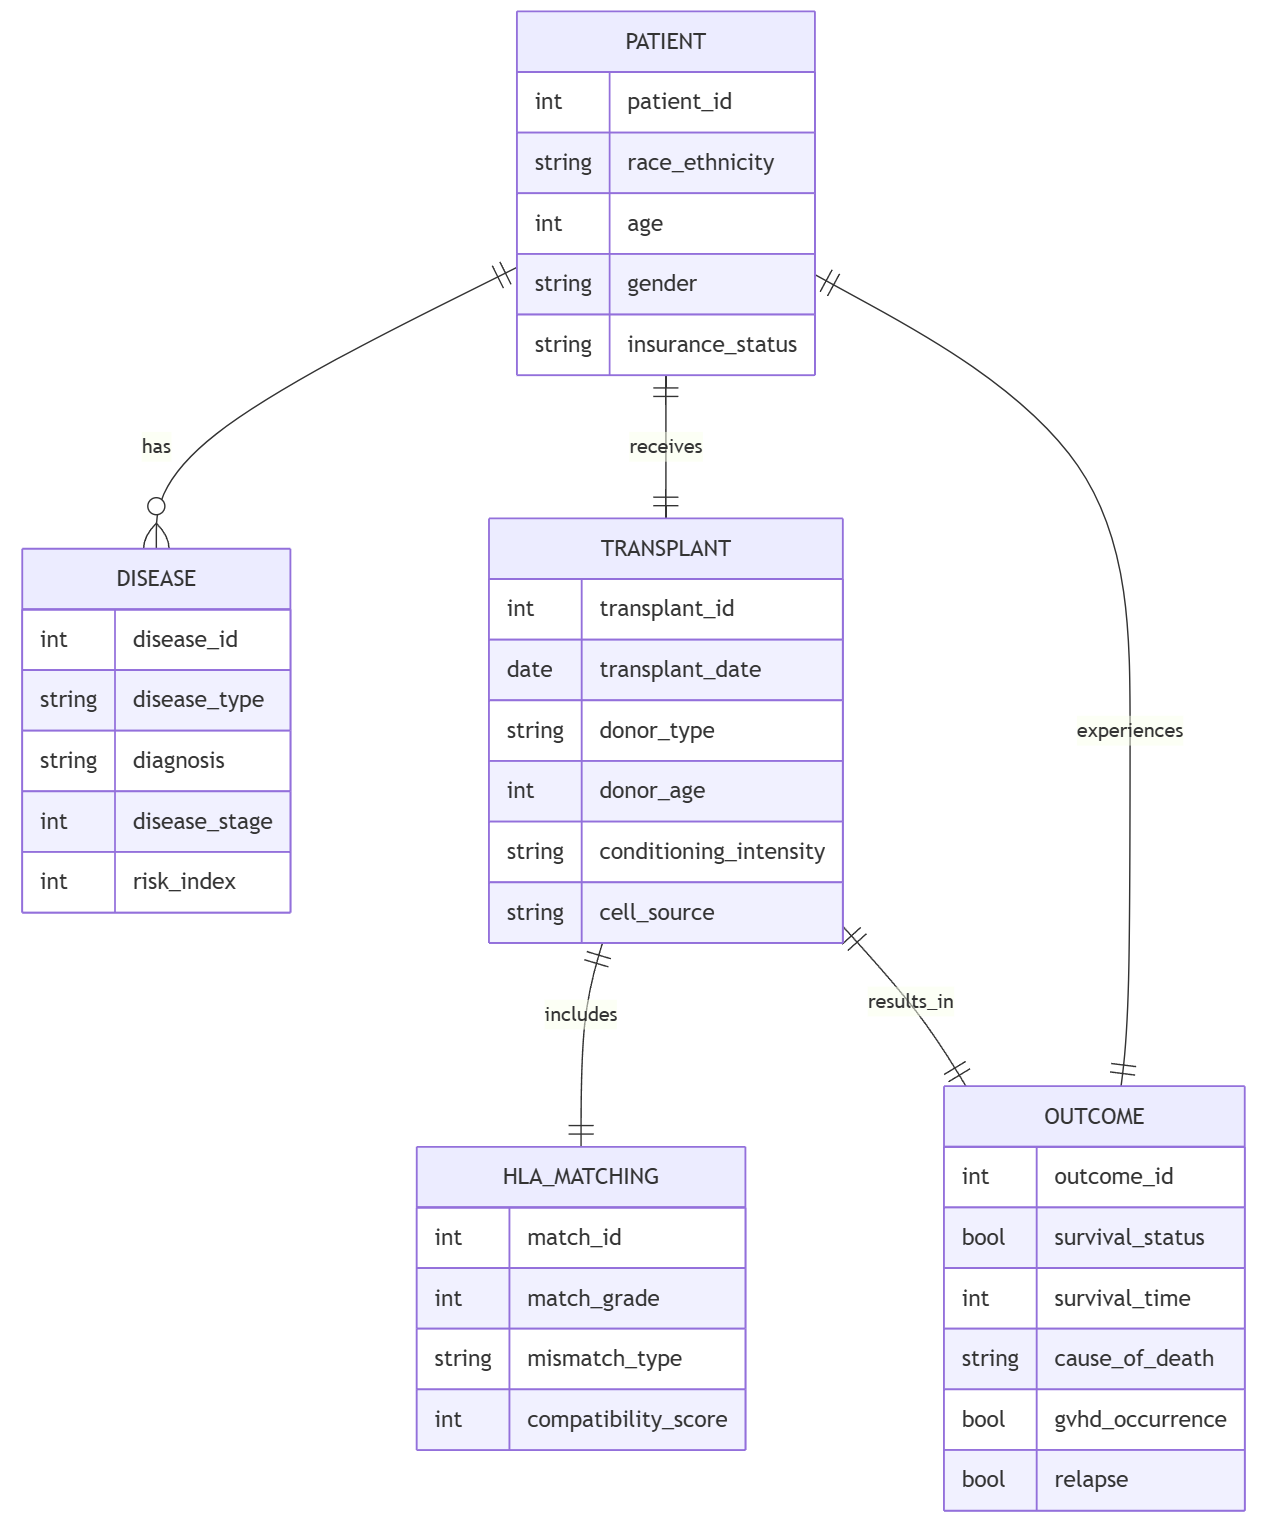
\includegraphics[width=0.4\textwidth]{figures/DataEntityRelationship.png}
    \caption{Entity-relationship diagram of the CIBMTR dataset structure showing the relationships between key data entities: patients, diseases, transplant procedures, HLA matching, and outcomes. This visualization maps how different data components are interconnected, highlighting the complexity of the dataset and providing context for the data constraints faced in prediction modeling.}
    \label{fig:data_er_diagram}
\end{figure}

\section{System Requirements}

\subsection{Measurable Design Requirements}

\begin{itemize}
    \item \textbf{Accuracy:} Production of results with the highest possible quality, enabling the fulfillment of user-centered needs.
    
    \item \textbf{Resilience:} Ability to maintain acceptable performance despite variations in the quantity or quality of input variables established for the system. This allows the system to properly handle generated entropy.
    
    \item \textbf{Efficiency:} Reduction in the amount of time and system resources without losing the established homeostasis in the system.
    
    \item \textbf{Scalability:} Simplicity when increasing the amount of data entered into the system.
\end{itemize}

\subsection{User-Centric Needs}

\begin{itemize}
    \item \textbf{Accuracy in post-HCT survival prediction}
    
    \item \textbf{Equity:} The model should not discriminate based on demographic or socioeconomic characteristics.
    
    \item \textbf{System resilience:} To handle missing data, outliers, and biological variability.
\end{itemize}

\begin{figure}[H]
    \centering
    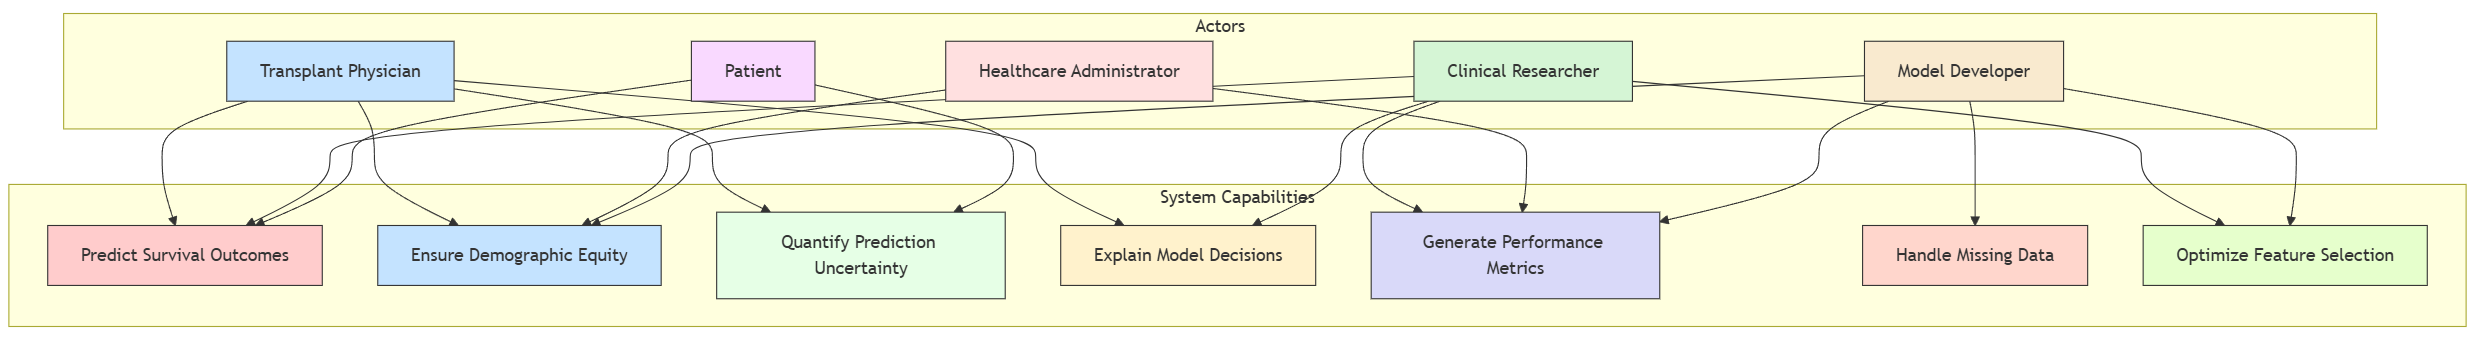
\includegraphics[width=0.95\textwidth]{figures/UseCaseDiagram.png}
    \caption{Use case diagram showing how different stakeholders interact with the prediction system. This visualization connects the technical capabilities of the system with the specific needs of transplant physicians, clinical researchers, healthcare administrators, model developers, and patients, illustrating how each user group utilizes different aspects of the system's functionality.}
    \label{fig:use_case_diagram}
\end{figure}

\begin{figure}[H]
    \centering
    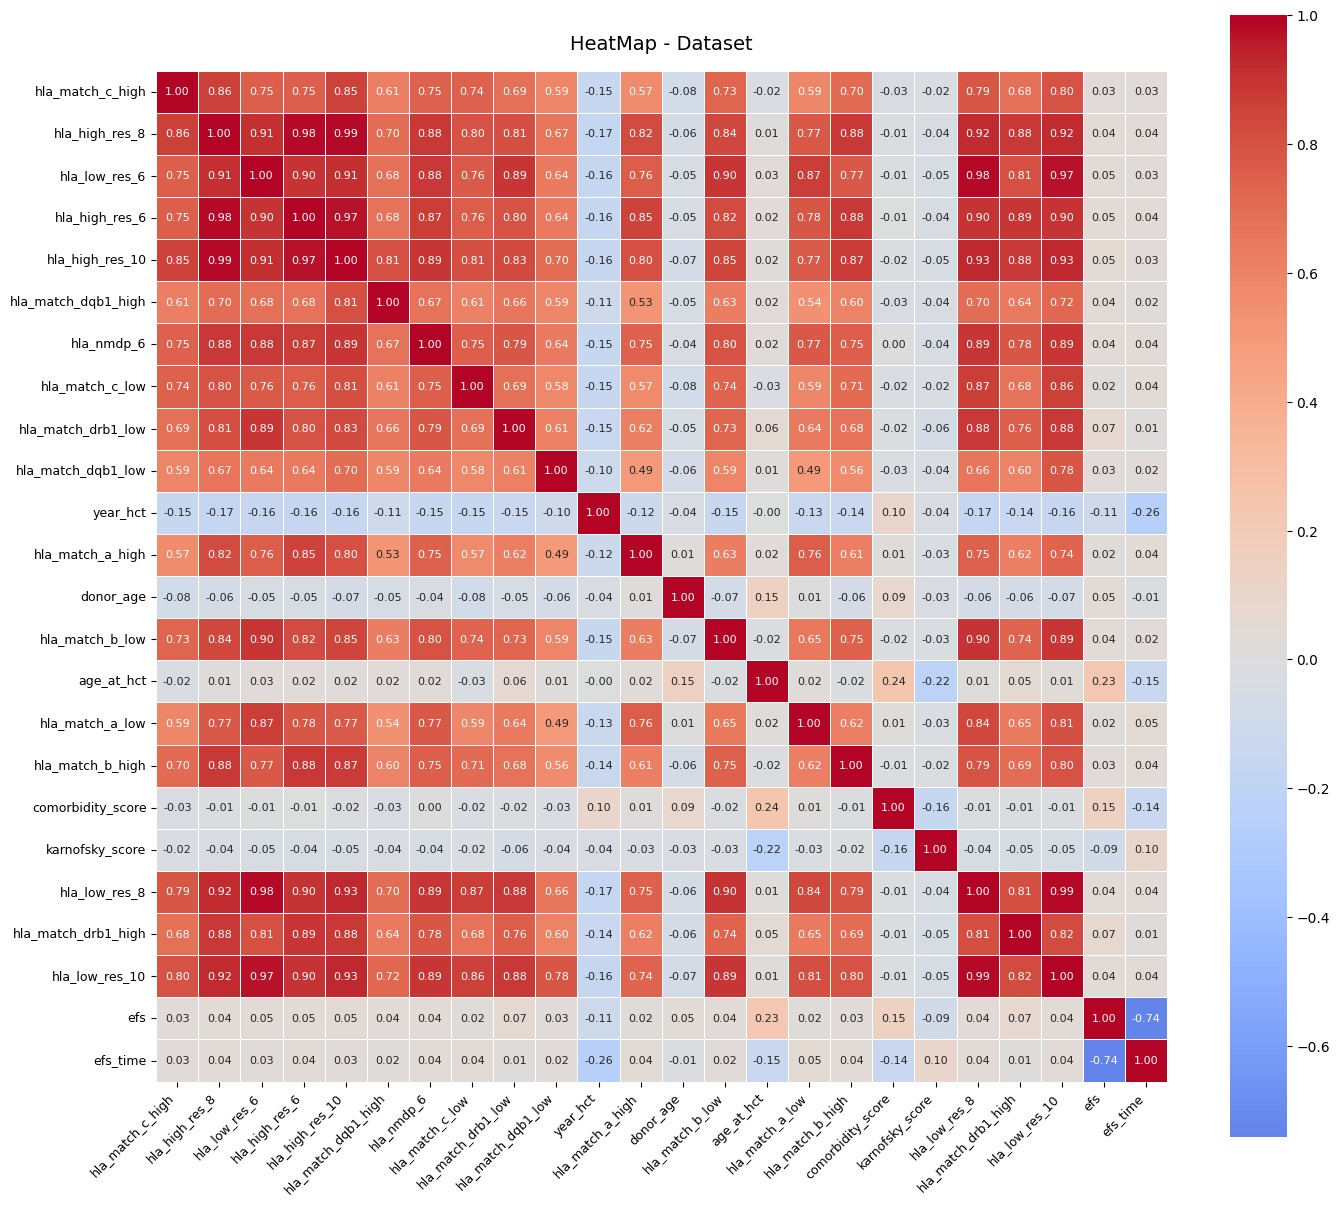
\includegraphics[width=1\textwidth]{figures/DatasetHeatmap.jpg}
    \caption{Heatmap visualization showing correlations between numerical variables in the dataset. This visualization facilitates understanding of the system's numerical input data to identify potential redundancies. By revealing which variables are highly correlated with each other, the heatmap provides insight into variable relationships that may influence system performance. This understanding allows us to prioritize relationships that contribute most effectively to the established system requirements, particularly with respect to equity considerations across demographic groups.}
    \label{fig:dataset_heatmap}
\end{figure}

\newpage

\subsection{Evaluation Metric and Fairness Assessment}

The stratified C-index serves as the primary evaluation metric for this system, designed specifically to ensure equity across demographic groups. This metric is central to the competition objectives and directly informs our architectural decisions.

\begin{figure}[H]
    \centering
    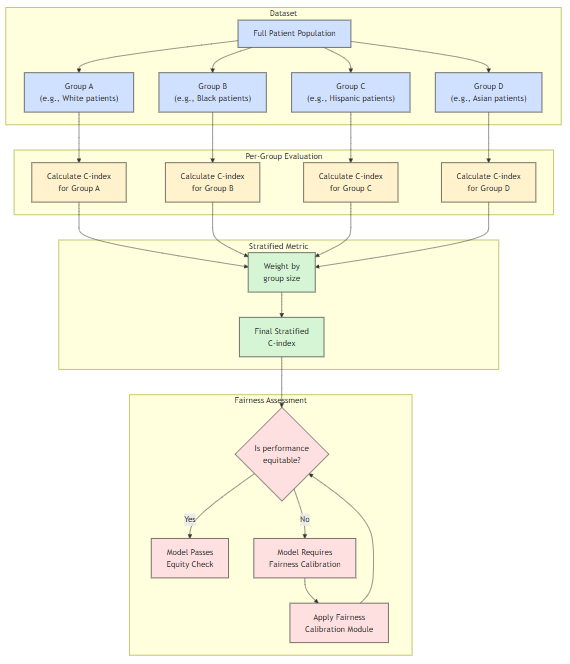
\includegraphics[width=0.95\textwidth]{figures/StratifiedCindexDiagram.png}
    \caption{Workflow for calculating the stratified C-index and performing fairness assessment. The process begins with stratification of the patient population by demographic groups, followed by separate C-index calculation within each group. These group-specific metrics are then weighted according to group size to produce the final stratified C-index. The fairness assessment loop ensures models deliver equitable performance across all patient populations, triggering fairness calibration when necessary.}
    \label{fig:cindex_fairness_diagram}
\end{figure}

This evaluation approach addresses a critical challenge in healthcare prediction: models may perform well on average while performing poorly for specific demographic groups. By requiring consistent performance across all patient populations, the stratified C-index incentivizes fair prediction systems that do not disadvantage underrepresented groups. Our architecture explicitly addresses this requirement through dedicated modules for equity analysis and fairness calibration.

\subsection{User Stories and Requirements Prioritization}

\subsubsection{User Stories}

We identified the following user stories to guide our system design:

\begin{itemize}
    \item \textbf{As a transplant physician}, I need accurate survival predictions stratified by demographic groups so that I can provide equitable prognostic information to all my patients regardless of their background.
    
    \item \textbf{As a clinical researcher}, I need to understand which factors most influence survival predictions so that I can identify potential interventions that might improve outcomes.
    
    \item \textbf{As a healthcare administrator}, I need performance metrics that demonstrate equitable model performance across populations so that I can ensure our institution delivers fair care.
    
    \item \textbf{As a model developer}, I need robust evaluation frameworks so that I can verify my algorithms maintain accuracy across different demographic subgroups.
    
    \item \textbf{As a patient}, I need trustworthy survival estimates with appropriate uncertainty bounds so that I can make informed decisions about my treatment options.
\end{itemize}

\subsubsection{Requirements Prioritization (MoSCoW)}

\begin{itemize}
    \item \textbf{Must Have:}
    \begin{itemize}
        \item Equity across demographic groups (measured by stratified C-index)
        \item Accurate survival predictions (minimum C-index of 0.70)
        \item Clinical validity of identified risk factors
        \item Appropriate uncertainty quantification
    \end{itemize}
    
    \item \textbf{Should Have:}
    \begin{itemize}
        \item Interpretability of model predictions
        \item Efficient computational performance
        \item Handling of complex missing data patterns
        \item Identification of potential biases in input data
    \end{itemize}
    
    \item \textbf{Could Have:}
    \begin{itemize}
        \item Integration capabilities with clinical workflows
        \item Advanced visualization of prediction uncertainty
        \item Personalization of risk thresholds
        \item Continuous learning capabilities
    \end{itemize}
    
    \item \textbf{Won't Have (This Version):}
    \begin{itemize}
        \item Integration with electronic health records
        \item Real-time prediction updates
        \item Patient-facing interfaces
        \item External data augmentation
    \end{itemize}
\end{itemize}

\subsubsection{Requirements Traceability}

To ensure all requirements are properly addressed by our architecture, we map key requirements to specific system components:

\begin{table}[H]
\centering
\begin{tabular}{|p{4cm}|p{1.5cm}|p{1.5cm}|p{1.5cm}|p{1.5cm}|p{1.5cm}|p{1.5cm}|}
\hline
\textbf{Requirement} & \textbf{\footnotesize Preproc.} & \textbf{\footnotesize Equity Analysis} & \textbf{\footnotesize Feature Selection} & \textbf{\footnotesize Modeling} & \textbf{\footnotesize Fairness} & \textbf{\footnotesize Outputs} \\
\hline
Equity across groups & \checkmark & \checkmark & \checkmark & \checkmark & \checkmark & \checkmark \\
\hline
Clinical interpretability & \checkmark & & \checkmark & & & \checkmark \\
\hline
Handling missing data & \checkmark & \checkmark & & & & \\
\hline
Uncertainty estimation & & & & \checkmark & \checkmark & \checkmark \\
\hline
Fairness across demographics & \checkmark & \checkmark & \checkmark & & \checkmark & \checkmark \\
\hline
\end{tabular}
\caption{Requirements traceability matrix showing how each system component addresses specific user and technical requirements. This visualization ensures all requirements are properly addressed within the system architecture.}
\label{tab:req_trace_matrix}
\end{table}

\section{High-Level Architecture}

\subsection{Architectural Overview}

The system architecture is founded on a modular and sequential pipeline that aims to optimize clinical accuracy and equity, responding to the complexity and high sensitivity identified in Workshop No. 1.

The architecture of the system is organized into modules representing the main stages, from the ingestion of raw data (clinical, genetic, and demographic data) to the generation of predictions and equity metrics for clinical decision support.

\begin{figure}[H]
    \centering
    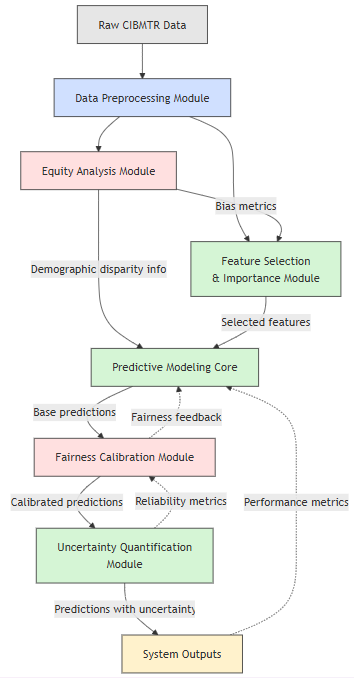
\includegraphics[width=0.5\textwidth]{figures/SystemArchitectureFlowchart.png}
    \caption{System architecture flowchart showing the seven core modules, data flow between components, and feedback loops. The arrows indicate the primary information flow, while dotted lines represent feedback mechanisms that enable continuous optimization. This design explicitly incorporates equity considerations throughout the prediction pipeline, with color-coding to distinguish different functional areas: blue for preprocessing, red for equity-focused components, green for modeling, and yellow for system outputs.}
    \label{fig:system_architecture_flowchart}
\end{figure}

\begin{figure}[H]
    \centering
    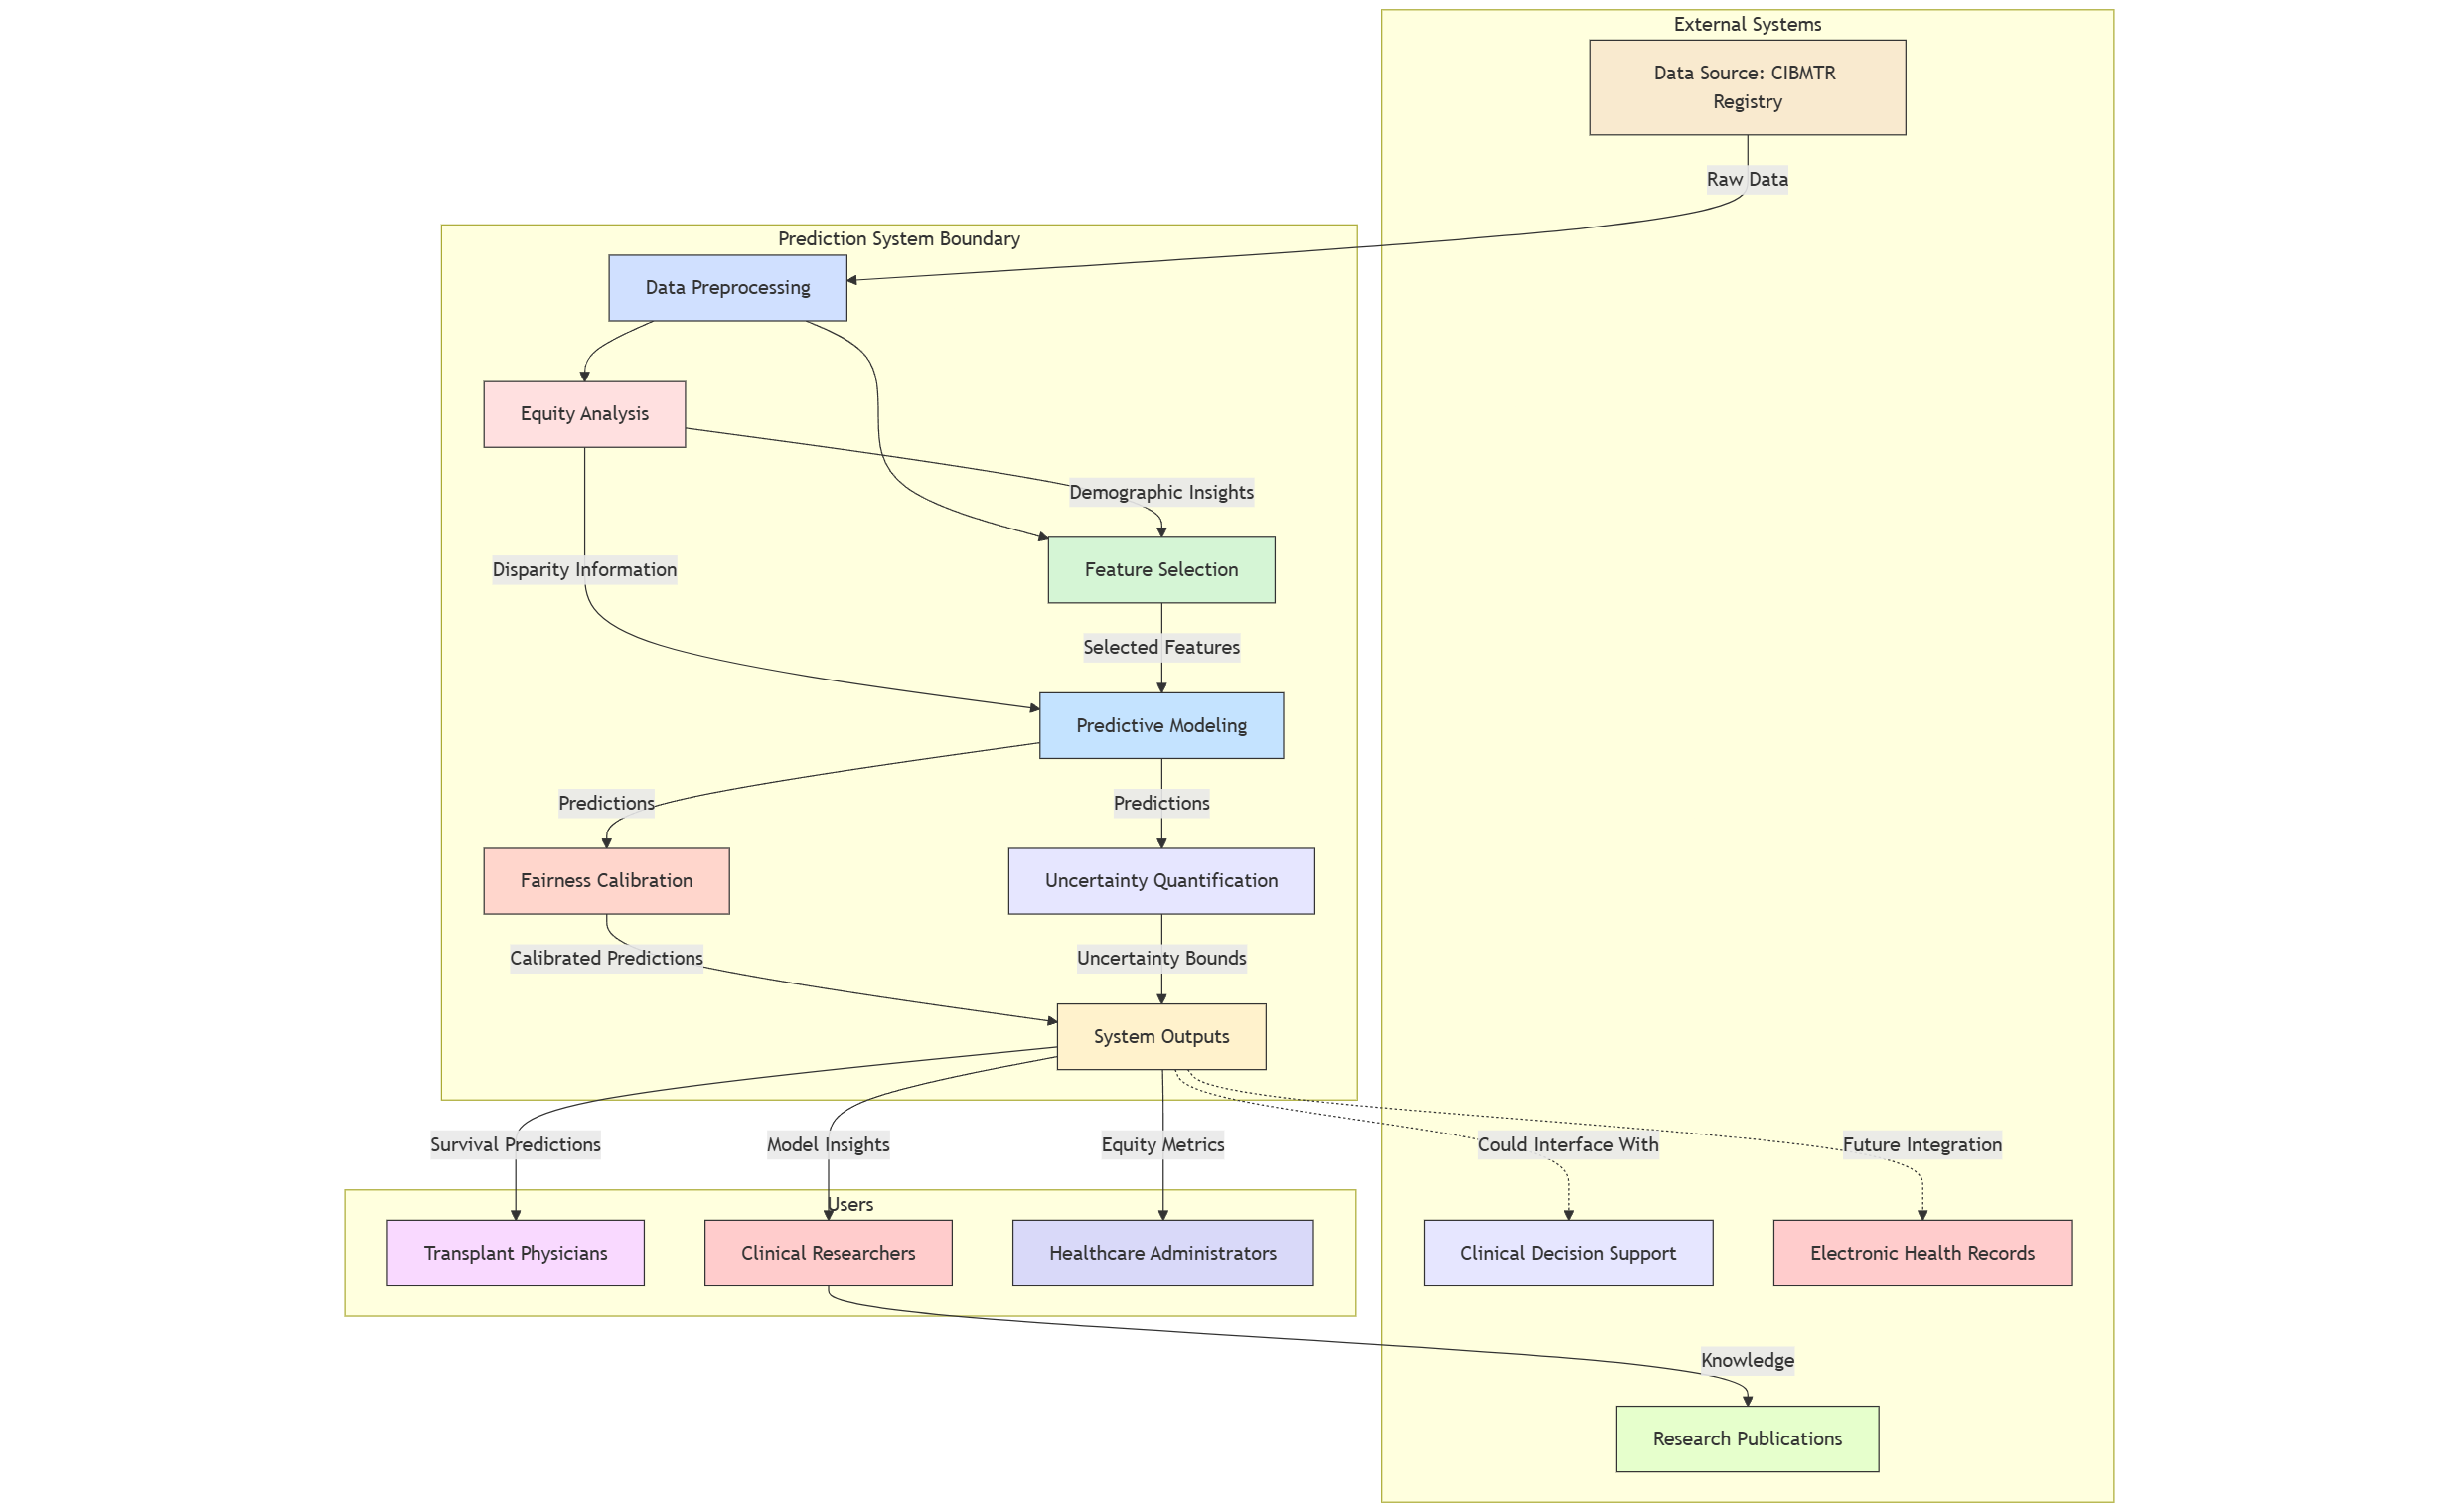
\includegraphics[width=1\textwidth]{figures/SystemContextDiagram.png}
    \caption{System context diagram showing the prediction system's boundaries and its interactions with external entities. The central area represents components within our system boundary, while external systems (data sources, clinical decision support) and users (physicians, researchers, administrators) are positioned outside. This visualization clarifies what is within the scope of our system versus what it interfaces with externally.}
    \label{fig:system_context_diagram}
\end{figure}

\subsection{Modules and Responsibilities}

The architecture consists of seven interconnected modules, each with a specific responsibility:

\subsubsection{1. Data Preprocessing Module}

\begin{table}[H]
\centering
\begin{tabular}{|p{5cm}|p{9cm}|}
\hline
\textbf{Internal Component} & \textbf{Specific Operations} \\
\hline
Ingestion and Validation & Verifies the integrity and format of raw CIBMTR data. \\
\hline
Equity-Aware Imputation & Handles missing and atypical data. Uses methods that consider demographic variations. \\
\hline
Standardization and Normalization & Scales and transforms continuous variables (e.g., Age, laboratory values) for ML models. \\
\hline
Basic Feature Engineering & Creation of interaction features and logarithmic transformation for skewed variables. \\
\hline
\end{tabular}
\caption{Data Preprocessing Module Components and Operations}
\label{tab:preprocessing_module}
\end{table}

\subsubsection{2. Equity Analysis Module}

\begin{table}[H]
\centering
\begin{tabular}{|p{5cm}|p{9cm}|}
\hline
\textbf{Internal Component} & \textbf{Specific Operations} \\
\hline
Stratified Analysis & Performs comprehensive examination of data in demographic subgroups (e.g., Race/Ethnicity) to identify disparities in baseline outcome rates. \\
\hline
Bias Detection Algorithms & Applies algorithms to measure bias in the quality or availability of input features. \\
\hline
Balancing Techniques & Uses fairness-aware preprocessing techniques such as reweighting to improve balanced representation. \\
\hline
\end{tabular}
\caption{Equity Analysis Module Components and Operations}
\label{tab:equity_module}
\end{table}

\subsubsection{3. Feature Selection and Importance Module}

\begin{table}[H]
\centering
\begin{tabular}{|p{5cm}|p{9cm}|}
\hline
\textbf{Internal Component} & \textbf{Specific Operations} \\
\hline
Clinical Domain Integration & Prioritizes sensitive variables identified (Age, Disease Risk Index, Genetic Compatibility). \\
\hline
ML/Statistical Rankings & Ranks feature importance using methods such as Recursive Feature Elimination or statistical significance. \\
\hline
Equitable Availability Verification & Ensures that critical predictive features are consistently available across all populations. \\
\hline
\end{tabular}
\caption{Feature Selection and Importance Module Components and Operations}
\label{tab:feature_module}
\end{table}

\subsubsection{4. Predictive Modeling Core}

\begin{table}[H]
\centering
\begin{tabular}{|p{5cm}|p{9cm}|}
\hline
\textbf{Internal Component} & \textbf{Specific Operations} \\
\hline
Proportional Hazards Models (Cox) & Base models for time-to-event survival predictions. \\
\hline
Ensemble Algorithms & Uses Gradient Boosting Machines (GBMs) and Random Forests to capture non-linear patterns. \\
\hline
Deep Learning Architectures & Implements neural models for complex non-linear relationships, when necessary. \\
\hline
Cross-Validation Strategy & Executes demographically stratified cross-validation adapted for survival data. \\
\hline
\end{tabular}
\caption{Predictive Modeling Core Components and Operations}
\label{tab:modeling_module}
\end{table}

\subsubsection{5. Fairness Calibration Module}

\begin{table}[H]
\centering
\begin{tabular}{|p{5cm}|p{9cm}|}
\hline
\textbf{Internal Component} & \textbf{Specific Operations} \\
\hline
Probability Calibration & Adjusts survival curves to maintain comparable accuracy across different patient populations. \\
\hline
Risk Threshold Optimization & Modifies risk classification thresholds (low, intermediate, high) to minimize disparity in risk assessment. \\
\hline
Disparity Impact & Quantifies the effect of adjustments to ensure minimization of prediction inequities. \\
\hline
\end{tabular}
\caption{Fairness Calibration Module Components and Operations}
\label{tab:fairness_module}
\end{table}

\subsubsection{6. Uncertainty Quantification Module}

\begin{table}[H]
\centering
\begin{tabular}{|p{5cm}|p{9cm}|}
\hline
\textbf{Internal Component} & \textbf{Specific Operations} \\
\hline
Prediction Interval Calculation & Generates confidence intervals using methods appropriate for survival analysis. \\
\hline
Risk and Reliability & Associates uncertainty bounds with risk stratification. \\
\hline
Low Reliability Identification & Flags cases where prediction is less reliable due to incomplete or atypical data. \\
\hline
\end{tabular}
\caption{Uncertainty Quantification Module Components and Operations}
\label{tab:uncertainty_module}
\end{table}

\subsubsection{7. System Outputs}

\begin{table}[H]
\centering
\begin{tabular}{|p{5cm}|p{9cm}|}
\hline
\textbf{Internal Component} & \textbf{Specific Operations} \\
\hline
Prediction Generator & Produces survival probabilities and risk stratification categories. \\
\hline
Equity Metrics Dashboard & Displays equity assessment and prediction consistency across groups. \\
\hline
Interpretation Engine (SHAP) & Generates detailed explanations for individual predictions (SHAP values, Feature Importance). \\
\hline
Quality and QA Reports & Delivers performance metrics, calibration plots, and data quality reports. \\
\hline
\end{tabular}
\caption{System Outputs Components and Operations}
\label{tab:outputs_module}
\end{table}

\subsection{System Information Flow}

To complement the modular architecture description, we visualize the temporal progression of information through the system with a sequence diagram:

\begin{figure}[H]
    \centering
    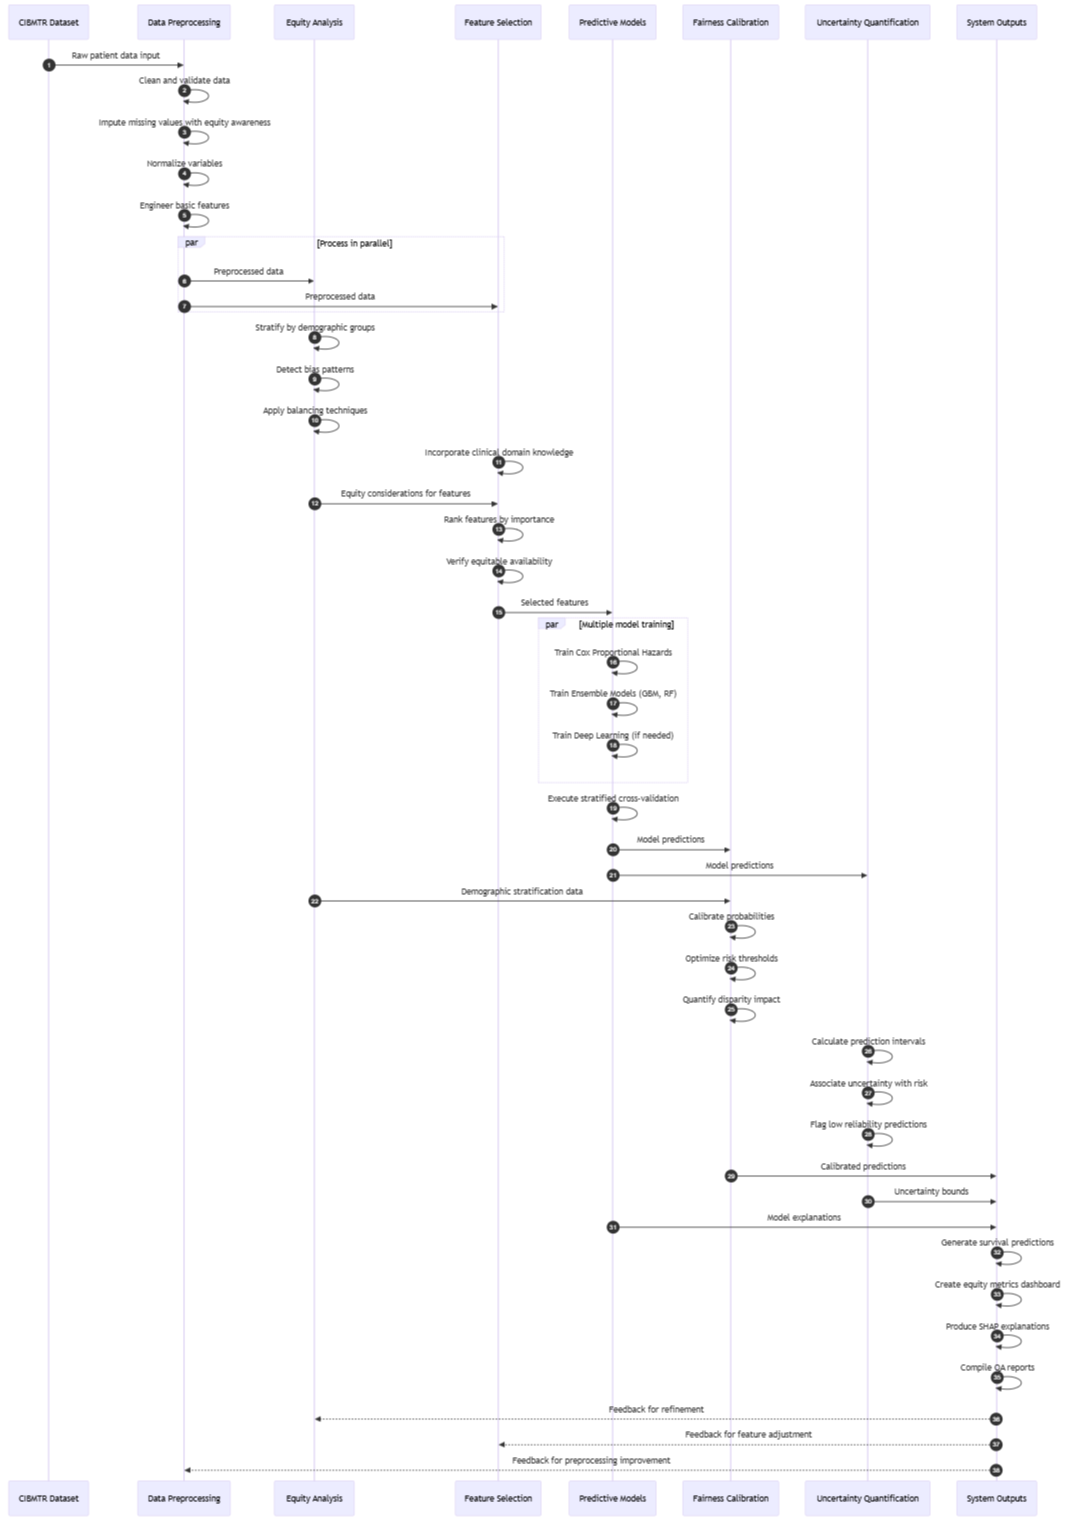
\includegraphics[width=1\textwidth]{figures/SystemSequenceDiagram.png}
    \caption{Detailed sequence diagram illustrating the flow of information through the system pipeline. The diagram shows how data progresses from the CIBMTR dataset through each processing stage, with parallel operations where appropriate and feedback loops enabling continuous improvement. Each numbered step represents a specific operation in the prediction workflow, highlighting the dynamic interactions between modules.}
    \label{fig:system_sequence_diagram}
\end{figure}

This sequence view demonstrates how information flows through our modules over time, including:
\begin{itemize}
    \item Parallel processing paths for efficiency
    \item Key decision points in the pipeline
    \item Feedback mechanisms that enable system learning and adaptation
    \item Sequential dependencies between operations
\end{itemize}

The diagram reinforces how equity considerations permeate the entire workflow, from initial data preprocessing through final output generation, ensuring fairness is maintained throughout the prediction process.

\subsection{Systems Engineering Principles}

The systems engineering principles applied to shape these structural decisions are:

\begin{itemize}
    \item \textbf{Modularity:} The architecture is divided into discrete modules, allowing independent development, testing, and component replacement without affecting overall system integrity.
    
    \item \textbf{Scalability:} The pipeline design supports complex methods such as ensemble modeling and stratified analysis. This ensures the system can handle both the high volume of data from CIBMTR and the computational complexity required.
    
    \item \textbf{Maintainability:} Clear documentation and separation of tasks are integrated. This separation facilitates audits and updates in response to new medical advances or equity requirements.
    
    \item \textbf{Robustness and Complexity Management:} 
    \begin{itemize}
        \item The inclusion of the Uncertainty Quantification Module and the use of ensemble models mitigate the effects of chaotic behavior and high system sensitivity (where small changes in input generate large changes in output).
        \item The Fairness Calibration Module reinforces system robustness against latent biases and ensures that the critical stratified C-Index metric is consistently met across all populations.
    \end{itemize}
\end{itemize}

\subsection{Complexity and Sensitivity Analysis}

\subsubsection{Complexity in Post-HCT Survival Modeling}

The challenge of predicting survival outcomes after hematopoietic cell transplantation (HCT) centers fundamentally on the system's inherent complexity \cite{astct_simplification}. Multiple interconnected clinical, genetic, and demographic factors influence patient survival outcomes, creating a nonlinear, high-dimensional system where minor parameter variations can produce significant outcome differences \cite{frontiers_ai_hct}.

As identified in our analysis, post-HCT survival prediction involves:

\begin{itemize}
    \item Multifactorial disease characteristics that vary by hematologic malignancy type \cite{ash_transplant_all}
    \item Complex donor-recipient genetic compatibility factors affecting engraftment \cite{mdpi_cells}
    \item Demographic variables with potential impact on healthcare access and outcomes \cite{jama_ai_medicine}
    \item Temporal aspects reflecting evolving medical practices over the dataset's time span \cite{mdpi_cancers}
\end{itemize}

Feedback mechanisms such as immune responses, graft-versus-host disease, and intervention-triggered complications further complicate prediction by introducing additional nonlinearity \cite{ash_chronic_gvhd}.

\subsubsection{Sensitivity Analysis}

Our analysis identified several parameters where small variations generate disproportionate impact on survival predictions:

\begin{itemize}
    \item \textbf{Age:} Even a single-year difference can shift risk categorization significantly for patients near clinical thresholds \cite{stmcls_clonality}
    \item \textbf{Disease risk indices:} Minor score changes can alter treatment eligibility and prognosis \cite{uptodate_hct}
    \item \textbf{HLA matching:} Subtle genetic compatibility differences substantially affect transplant rejection rates \cite{frontiers_immunology}
    \item \textbf{Comorbidities:} Presence or absence of specific conditions can dramatically alter survival projections \cite{mdpi_cancers}
\end{itemize}

\begin{figure}[H]
    \centering
    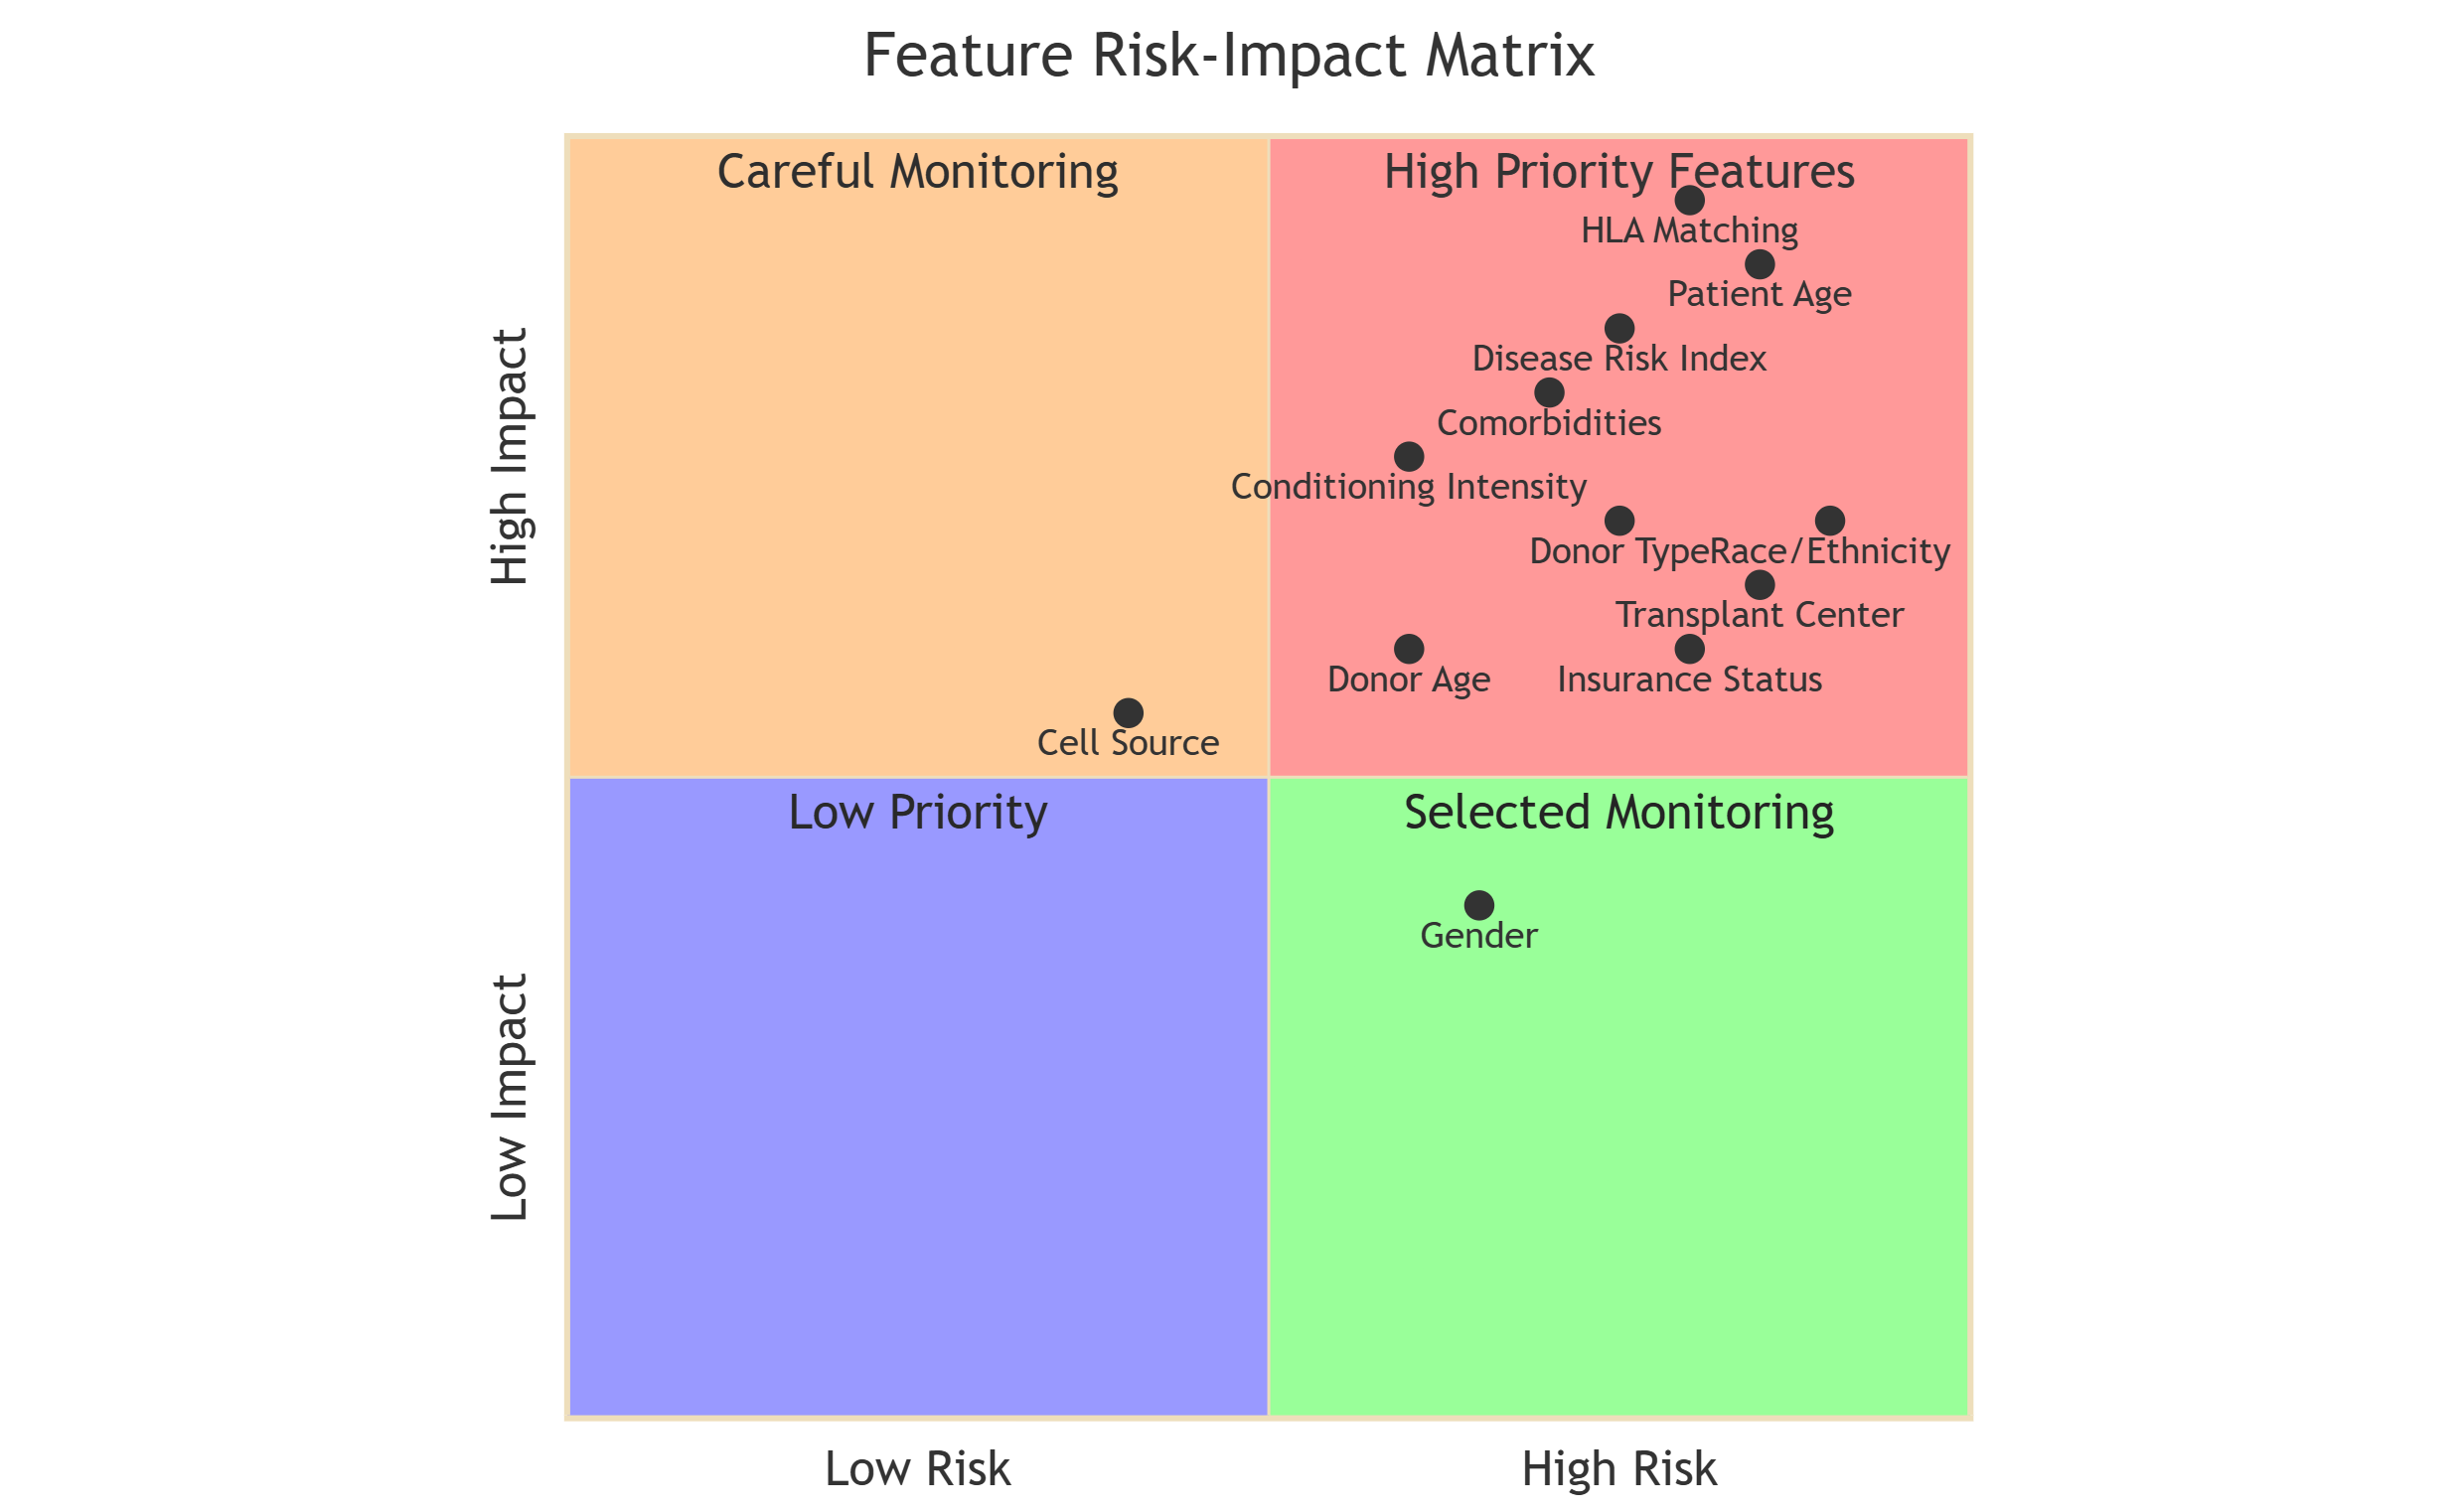
\includegraphics[width=0.6\textwidth]{figures/RiskImpactMatrix.png}
    \caption{Risk-impact matrix for key prediction features, positioning variables according to their predictive power (impact) and potential for introducing bias (risk). High-impact, high-risk features like patient age and HLA matching require particular attention in our fairness calibration process. This visualization guides our feature selection strategy by highlighting which variables need careful handling to balance predictive power against equity considerations.}
    \label{fig:risk_impact_matrix}
\end{figure}

\begin{figure}[H]
    \centering
    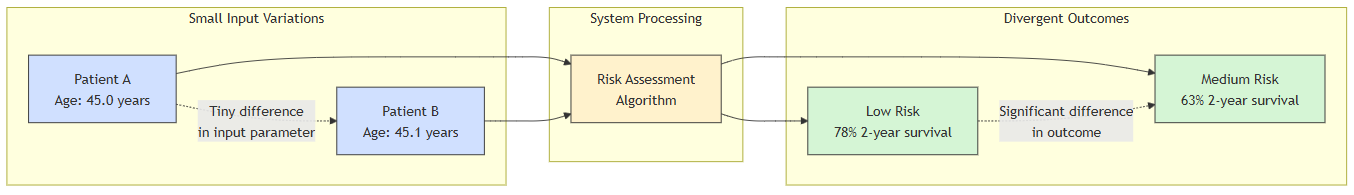
\includegraphics[width=0.95\textwidth]{figures/SensitivityDiagram.png}
    \caption{Visual representation of sensitivity in post-HCT survival prediction. This diagram illustrates how a minimal difference in patient age (just 0.1 years) can lead to significantly different risk categorization and survival probability estimates. Such high sensitivity to input parameters necessitates specialized modeling approaches that can account for these threshold effects, particularly around clinical decision boundaries.}
    \label{fig:sensitivity_diagram}
\end{figure}

\subsubsection{Chaos and Randomness in Post-HCT Survival Prediction}

Medical outcomes following allogeneic HCT exhibit characteristics of chaotic systems, where deterministic processes nonetheless produce seemingly random and unpredictable results \cite{frontiers_ai_hct}. This chaos manifests in several specific ways:

\begin{itemize}
    \item \textbf{Immune reconstitution dynamics:} Small variations in initial T-cell populations can lead to dramatically different immune recovery trajectories and corresponding survival outcomes \cite{stmcls_clonality}. Studies show that even genetically identical grafts can produce divergent immune reconstitution patterns due to sensitivity to microenvironmental conditions at transplantation.
    
    \item \textbf{Graft-versus-host disease emergence:} The development and progression of GVHD follows chaotic patterns, with similar patients on identical prophylaxis regimens experiencing vastly different disease trajectories \cite{ash_chronic_gvhd}. Minor differences in tissue damage during conditioning or subtle variations in gut microbiota can trigger significantly different inflammatory cascades.
    
    \item \textbf{Infection susceptibility:} Infection outcomes post-transplant display hallmarks of chaos theory, where minimal differences in pathogen exposure or antimicrobial timing can result in either rapid clearance or life-threatening sepsis \cite{uptodate_hct}.
    
    \item \textbf{Relapse dynamics:} For malignant conditions, disease recurrence follows complex nonlinear patterns influenced by minimal residual disease, graft-versus-leukemia effects, and immune escape mechanisms that exhibit extreme sensitivity to initial conditions \cite{mdpi_cancers}.
\end{itemize}

The ``butterfly effect'' in these systems means that conventional deterministic models struggle to capture the true range of possible outcomes. Our analysis revealed that this unpredictability is further complicated by demographic factors, as certain chaos-inducing variables (like access to prompt care for infections or monitoring for early GVHD signs) may be systematically distributed unequally across patient populations \cite{jama_ai_medicine}.

The competition's stratified C-index evaluation metric \cite{kaggle_competition} presents a particular challenge in this context, as it requires models to maintain consistent performance across demographic subgroups despite these chaotic elements. Achieving both accuracy and equity demands sophisticated approaches that can:

\begin{itemize}
    \item Quantify uncertainty ranges rather than single-point predictions
    \item Identify regions of the feature space where chaotic behavior is most likely
    \item Apply ensemble methods that capture various possible trajectory families
    \item Maintain calibration across demographic groups even when faced with inherent unpredictability
\end{itemize}

These considerations directly inform our system design, which employs multiple modeling approaches and explicit uncertainty quantification to address the fundamental chaotic nature of post-HCT outcomes while ensuring equitable performance across patient populations.

\section{Technical Stack and Implementation Sketch}

We have identified a range of widely-used and accessible tools designed to handle everything from data cleaning to results presentation, ensuring that the work can be replicated without difficulties.

\subsection{Recommended Technology Stack}

\subsubsection{Data Processing and Management Tools}

\begin{itemize}
    \item \textbf{Pandas:} Enables efficient organization and cleaning of information, such as sorting patient tables or transforming medical data \cite{geeksforgeeks_pandas}.
    
    \item \textbf{NumPy:} Facilitates rapid calculations and matrix operations, supporting all statistical processing needs \cite{dataquest_numpy}.
    
    \item \textbf{Scikit-learn:} Provides functions for data preparation, filling missing values, and splitting information for model training and validation \cite{pushkarna_preprocessing}.
\end{itemize}

\subsubsection{Survival Analysis Libraries}

\begin{itemize}
    \item \textbf{Lifelines:} This library assists in analyzing patient survival time. It includes models such as Cox Proportional Hazards and methods to calculate expected time to an event using available information \cite{lifelines_docs}.
    
    \item \textbf{Scikit-survival:} Enables the use of more advanced survival models and is compatible with other machine learning tools, making the process simpler and more integrated \cite{scikit_survival_intro}.
\end{itemize}

\subsubsection{Machine Learning Models}

\begin{itemize}
    \item \textbf{XGBoost:} Very fast and works well with large data volumes. Additionally, it detects missing values and adjusts calculations if there are fewer cases in one group than another \cite{neptune_boosting}.
    
    \item \textbf{LightGBM:} Consumes less memory than other options and has faster training times, ideal for working with many records \cite{cienciadedatos_forecast}.
    
    \item \textbf{CatBoost:} Allows direct use of categorical data without prior conversion, saving time and reducing errors \cite{geeksforgeeks_boosting}.
\end{itemize}

\subsubsection{Fairness and Bias Reduction Tools}

\begin{itemize}
    \item \textbf{AIF360 (IBM):} Allows fairness measurement using various metrics and applies techniques to reduce bias either before, during, or after model training \cite{aif360_github}.
    
    \item \textbf{Fairlearn (Microsoft):} Offers options to adjust models and ensure results are fair across all groups \cite{fairlearn_org}.
\end{itemize}

\subsubsection{Model Interpretation Tools}

\begin{itemize}
    \item \textbf{SHAP:} Used to explain, through graphics and values, why the model makes certain decisions \cite{shap_intro}.
\end{itemize}

\subsubsection{Data Visualization}

\begin{itemize}
    \item \textbf{Matplotlib:} Creates basic or advanced charts to clearly display analysis results \cite{matplotlib_org}.
    
    \item \textbf{Seaborn:} Enables creation of more attractive and easier-to-interpret statistical graphics, quickly comparing groups or trends \cite{seaborn_org}.
\end{itemize}

\subsubsection{Technical Management and Deployment}

\begin{itemize}
    \item \textbf{Docker:} Ensures the project works identically on any computer, avoiding configuration-related errors \cite{kdnuggets_pipeline}.
    
    \item \textbf{PostgreSQL:} Stores all data and results to keep history secure and organized.
    
    \item \textbf{MLflow:} Records experiments and results of each model version for easy comparison and selection of the best option \cite{datacamp_mlops}.
\end{itemize}

\subsection{Implementation Approach}

\subsubsection{Development Methodology}

\begin{figure}[H]
    \centering
    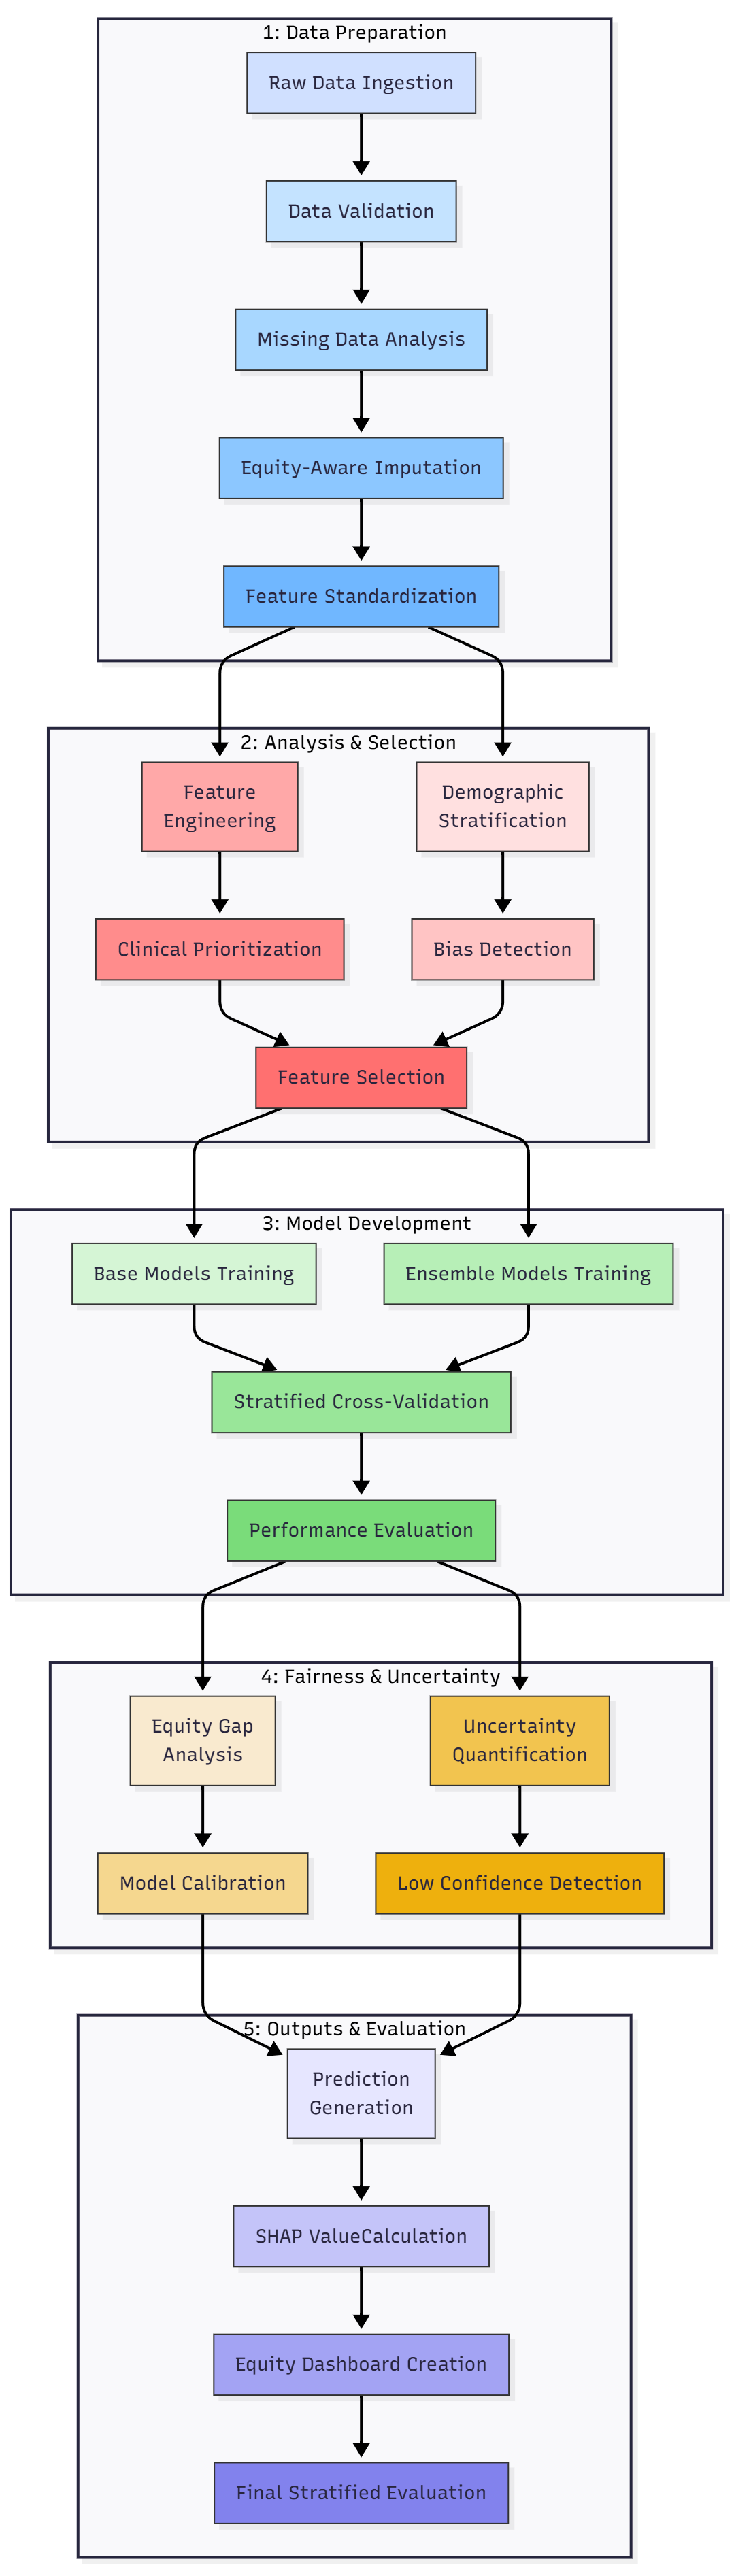
\includegraphics[width=0.35\textwidth]{figures/DevelopmentWorkflow.png}
    \caption{Development workflow diagram showing the five implementation phases: Data Preparation, Analysis \& Selection, Model Development, Fairness \& Uncertainty, and Outputs \& Evaluation. Each phase contains specific tasks that must be completed before progressing to subsequent phases, though feedback loops exist between phases for iterative refinement. Color-coding distinguishes different phases of implementation, highlighting both the sequential nature of development and cross-phase dependencies.}
    \label{fig:development_workflow}
\end{figure}

Our implementation will follow a structured workflow that addresses both the technical challenges of accurate prediction and the ethical requirements for equity:

\begin{enumerate}
    \item \textbf{Data Preparation:} First, missing data is cleaned and completed, ensuring fair treatment across different groups such as race or ethnicity. Then, values are normalized so all patients are on the same scale.
    
    \item \textbf{Fairness Analysis:} Using AIF360, information is converted to a special format and metrics like ``Statistical Parity Difference'' are calculated to determine if the system treats all groups fairly.
    
    \item \textbf{Feature Selection:} The most important variables are chosen using statistical methods and ensemble models that detect which factors most affect survival.
    
    \item \textbf{Predictive Modeling:} Several models are trained, including ``Cox Proportional Hazards'', ``Gradient Boosting Survival Analysis'', and XGBoost, adjusting parameters when there are fewer cases in some groups.
    
    \item \textbf{Fairness Calibration:} Techniques are applied to correct bias after training the model and adjust thresholds to ensure predictions are fair across groups.
    
    \item \textbf{Uncertainty Quantification:} Confidence intervals are calculated to determine how certain the model is in its predictions, using repeated simulations (bootstrap).
    
    \item \textbf{System Output Generation:} A visual explanation of each prediction is generated with SHAP, showing why the model decides in a particular way and which features have the most influence.
\end{enumerate}

\subsubsection{Design Patterns}

The implementation incorporates several design patterns to ensure maintainability and scalability:

\begin{itemize}
    \item \textbf{Pipeline Pattern:} All process steps are connected to automate and avoid errors when processing data \cite{datacamp_mlops}.
    
    \item \textbf{Strategy Pattern:} The cleaning method, prediction model, or equity techniques can be changed depending on what the study seeks to achieve.
    
    \item \textbf{Observer Pattern:} With MLflow, every change and result is automatically recorded to monitor the process.
\end{itemize}

\subsubsection{Implementation Considerations}

\begin{itemize}
    \item \textbf{Cross-Validation:} To ensure consistent results, data is divided into several groups, mixing the event of interest (such as survival) and demographic characteristics. The model is trained multiple times, and performance in each group is compared using the C-index \cite{scikit_learn_cv}.
    
    \item \textbf{Parallelization:} Computationally intensive processes like cross-validation and ensemble training are parallelized to improve efficiency.
    
    \item \textbf{Memory Management:} For large datasets, efficient memory management techniques are employed, particularly when working with ensemble models.
    
    \item \textbf{Data Security:} Although using de-identified data, appropriate security controls are maintained throughout the implementation.
    
    \item \textbf{Reproducibility:} All random processes use fixed seeds to ensure reproducibility of results.
\end{itemize}

\section{Conclusion}

In this report, we have presented a comprehensive system design that addresses the dual challenges of accuracy and equity in post-HCT survival predictions identified in Workshop No. 1. Our architecture directly responds to the complex, sensitive, and chaotic nature of the medical domain while maintaining a focus on fair outcomes across demographic groups.

The proposed modular pipeline architecture, consisting of seven interconnected components, systematically addresses each aspect of the prediction challenge:

\begin{itemize}
    \item The Data Preprocessing and Equity Analysis modules establish a foundation for fairness from the earliest stages of data handling, ensuring demographic disparities are not amplified through the prediction pipeline.
    
    \item The Feature Selection and Importance Module prioritizes variables based on both clinical relevance and stability, with special attention to the high-sensitivity parameters identified in our analysis.
    
    \item The Predictive Modeling Core employs multiple complementary algorithms that collectively capture the nonlinear patterns essential for accurate survival prediction while mitigating the chaotic elements inherent in post-HCT outcomes.
    
    \item The Fairness Calibration Module provides explicit mechanisms to optimize the critical stratified C-index metric by ensuring consistent performance across demographic subgroups.
    
    \item The Uncertainty Quantification Module acknowledges and communicates the inherent unpredictability in medical outcomes, enhancing clinical trust and decision-making.
    
    \item The System Outputs module delivers not only predictions but explanations and equity metrics that support transparent and fair clinical application.
\end{itemize}

Our carefully selected technical stack balances state-of-the-art capabilities with practical implementation concerns, ensuring that the sophisticated modeling approaches required for this domain remain computationally feasible and reproducible.

\subsection{Limitations and Considerations}

Despite the comprehensive nature of our design, several important limitations and considerations must be acknowledged:

\begin{itemize}
    \item \textbf{Trade-offs between accuracy and interpretability:} While ensemble methods provide superior predictive performance, they can reduce interpretability compared to simpler models. Our design attempts to balance these concerns through SHAP-based explanations, but this tension remains fundamental to the problem domain.
    
    \item \textbf{Data constraints:} Working exclusively with the competition dataset limits our ability to incorporate potentially valuable external information. The system design includes robust handling of missing data, but cannot entirely overcome fundamental data limitations.
    
    \item \textbf{Computational complexity:} The sophisticated modeling approaches necessary for addressing the complex and chaotic nature of post-HCT outcomes require significant computational resources, potentially limiting real-time application in resource-constrained clinical settings.
    
    \item \textbf{Evolving clinical knowledge:} Medical understanding and practices in HCT continue to evolve, requiring regular updates to model parameters and potentially architectural changes to incorporate new prognostic factors.
    
    \item \textbf{Ethical dimensions beyond technical fairness:} While our design emphasizes statistical equity across demographic groups, broader ethical considerations in healthcare prediction extend beyond what can be addressed through technical means alone.
\end{itemize}

\subsection{Future Enhancements}

Looking beyond the current design, several promising directions for future enhancement emerge:

\begin{itemize}
    \item \textbf{Continuous learning systems:} Implementing a feedback loop that incorporates new patient outcomes to continuously refine and recalibrate predictions over time, adapting to evolving medical practices.
    
    \item \textbf{Expanded demographic considerations:} Extending equity analyses beyond the demographic factors in the current competition to address additional dimensions of potential healthcare disparities.
    
    \item \textbf{Federated learning approaches:} Developing techniques that allow model training across multiple transplant centers while preserving data privacy, significantly expanding available training data.
    
    \item \textbf{Temporal modeling improvements:} Incorporating more sophisticated approaches to capture the time-dependent nature of post-transplant complications and interventions.
    
    \item \textbf{Integration with electronic health records:} Creating interfaces between the prediction system and clinical workflows to facilitate seamless integration into transplant decision-making processes.
    
    \item \textbf{Patient-specific visualizations:} Developing personalized risk communication tools that effectively convey prediction uncertainty to support shared decision-making between clinicians and patients.
\end{itemize}

In summary, our system design represents a robust framework for addressing the complex challenges of equitable survival prediction following HCT. By explicitly addressing the sensitivity, chaos, and equity considerations identified in Workshop No. 1, this architecture provides a foundation for models that can deliver both accurate and fair predictions across diverse patient populations.
    
    % -------------------------------------------------------------------
    % Bibliography/References
    % -------------------------------------------------------------------
    \bibliography{references}  % Add entries for sources: academic papers, official documents, web pages.
    
\end{document}